% Copyright (c) Patrick Hall (jphall@gwu.edu), 2026-27. CC BY-NC-SA 4.0.
\documentclass[aspectratio=169]{beamer}
\usetheme{Singapore}
\definecolor{brand}{RGB}{45,110,191}
\definecolor{hrgray}{RGB}{100,100,100}
\definecolor{riskred}{RGB}{177,43,43}
\definecolor{safegreen}{RGB}{32,120,80}
\setbeamercolor{structure}{fg=brand}
\setbeamercolor{title}{fg=hrgray}
\setbeamercolor{subtitle}{fg=brand}
\setbeamercolor{frametitle}{fg=hrgray}
\setbeamercolor{block title}{fg=white,bg=brand}
\setbeamercolor{block body}{bg=black!2}
\usepackage[T1]{fontenc}
\usepackage[utf8]{inputenc}
\usepackage{lmodern,microtype,graphicx,booktabs,tabularx,array,tikz,amsmath}
\usepackage[backend=biber,style=authoryear,maxcitenames=2,maxbibnames=10,doi=false,isbn=false,url=true]{biblatex}
\addbibresource{references.bib}
\DeclareBibliographyCategory{referencesone}
\DeclareBibliographyCategory{referencestwo}
\DeclareBibliographyCategory{referencesthree}
\DeclareBibliographyCategory{referencesfour}
\addtocategory{referencesone}{adebayo2018sanity,alvarezmelis2018robustness,Amironesei2025AssessingRisksImpacts,artstein2008intercoder,Balloccu2024LeakCheatRepeat,campbell1959convergent}
\addtocategory{referencestwo}{Chen2021EvaluatingLargeLanguage,cronbach1955construct,Ganguli2022RedTeamingReduceHarms,geifman2017selective,Hendrycks2021MeasuringMassiveMultitask,ieee1012-2024}
\addtocategory{referencesthree}{Liu2023GEval,messick1987validity,nasa2017handbook,NationalInstituteStandards2023ArtificialIntelligenceRisk,Perez2022RedTeamingLanguage,Phillips2026TEVVAthlon,Reimers2019SentenceBERT}
\addtocategory{referencesfour}{Thomas2022RelianceMetricsFundamental,Wallach2024EvaluatingGenerativeAi,Weidinger2023SociotechnicalSafetyEvaluation,yeh2019infidelity,zheng2023judging}
\renewcommand*{\mkbibacro}[1]{#1}
\renewcommand*{\bibfont}{\scriptsize}
\usetikzlibrary{positioning,arrows.meta,shapes.geometric,fit}
\setbeamertemplate{navigation symbols}{}
\setbeamertemplate{bibliography item}{}
\setbeamertemplate{frametitle continuation}{}
\setbeamertemplate{footline}{\leavevmode\hbox{\begin{beamercolorbox}[wd=.5\paperwidth,ht=3ex,dp=1ex,left]{author in head/foot}\hspace{0.8ex}
\includegraphics[height=.5cm]{../../asset/gw_logo.png}\end{beamercolorbox}\begin{beamercolorbox}[wd=.5\paperwidth,ht=3ex,dp=1ex,right]{date in head/foot}\insertframenumber/\inserttotalframenumber\hspace{2ex}\end{beamercolorbox}}}
\title{Lecture 7: TEVV for LLM applications}
\subtitle{Testing, Evaluation, Verification and Validation for LLM Applications}
\author[Patrick Hall]{\textbf{Patrick Hall}}
\institute{Department of Decision Sciences}
\date{\today}
\newcommand{\slidesource}[1]{\vfill\tiny\color{hrgray}Source: #1.}
\newcommand{\visualdescription}[1]{\par\vspace{.2em}{\centering\tiny\color{hrgray}#1\par}}
\newcommand{\R}{\mathbb{R}}
\newcolumntype{Y}{>{\raggedright\arraybackslash}X}

\begin{document}

\begin{frame}
  \titlepage
  \vspace{-.75em}
  \centering\scriptsize \textcopyright\ 2026--27 Patrick Hall (jphall@gwu.edu). Some rights reserved. Text and copy are licensed under a \href{https://creativecommons.org/licenses/by-nc-sa/4.0/}{Creative Commons Attribution-NonCommercial-ShareAlike 4.0 International License (CC BY-NC-SA 4.0)}.
  \begin{tikzpicture}[remember picture,overlay]
    \node[opacity=.08] at (current page.center) {
\includegraphics[width=.55\paperwidth]{../../asset/gw_logo.png}};
  \end{tikzpicture}
\end{frame}

\begin{frame}{Agenda}
  \tableofcontents
\end{frame}

\section{Measurement foundations}

\begin{frame}{TEVV builds evidence for a decision}
\small
\centering
\vspace{.9em}
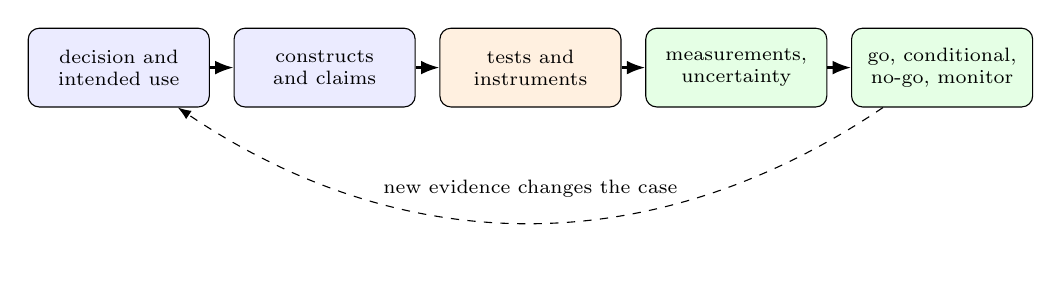
\begin{tikzpicture}[>=Latex,node distance=3mm,every node/.style={font=\scriptsize,align=center}]
  \node[draw,rounded corners,fill=blue!8,minimum width=23mm,minimum height=10mm] (goal) {decision and\\intended use};
  \node[draw,rounded corners,fill=blue!8,minimum width=23mm,minimum height=10mm,right=of goal] (construct) {constructs\\and claims};
  \node[draw,rounded corners,fill=orange!12,minimum width=23mm,minimum height=10mm,right=of construct] (test) {tests and\\instruments};
  \node[draw,rounded corners,fill=green!10,minimum width=23mm,minimum height=10mm,right=of test] (evidence) {measurements,\\uncertainty};
  \node[draw,rounded corners,fill=green!10,minimum width=23mm,minimum height=10mm,right=of evidence] (action) {go, conditional,\\no-go, monitor};
  \draw[->,thick] (goal)--(construct); \draw[->,thick] (construct)--(test);
  \draw[->,thick] (test)--(evidence); \draw[->,thick] (evidence)--(action);
  \draw[->,dashed,bend left=34] (action) to node[midway,above=2mm]{new evidence changes the case} (goal);
\end{tikzpicture}
\visualdescription{A decision-centered evidence chain connects intended use to constructs, instruments, measurements, and action, with monitoring feeding back into reassessment.}
\vspace{-.2em}
\begin{columns}[T]
\column{.48\textwidth}
\begin{block}{TEVV}
\textbf{Test} behavior; \textbf{evaluate} results against criteria; \textbf{verify} that requirements were implemented; \textbf{validate} fitness for the intended use.
\end{block}
\column{.48\textwidth}
\begin{block}{Central discipline}
Do not begin with a convenient score. Begin with the claim and decision the score must support.
\end{block}
\end{columns}
\slidesource{\parencite{Phillips2026TEVVAthlon}, \href{https://doi.org/10.6028/NIST.AI.200-2.ipd}{decision-centered, contextual TEVV}}
\end{frame}

\begin{frame}{Measurement connects evidence to governance}
\footnotesize
\begin{columns}[c]
\column{.48\textwidth}
\begin{itemize}
  \item \textbf{Context:} start with organizational goals, stakeholders, and lifecycle context.
  \item \textbf{Constructs:} define trustworthy characteristics as measurable constructs.
  \item \textbf{Instrument validation:} assess reliability, validity, sensitivity, and intended use.
  \item \textbf{Measurement:} apply tools through planned events.
  \item \textbf{Synthesis:} form evidence and qualified conclusions.
  \item \textbf{Governance:} use the evidence to support Govern, Map, and Manage decisions.
\end{itemize}
\column{.48\textwidth}
\centering
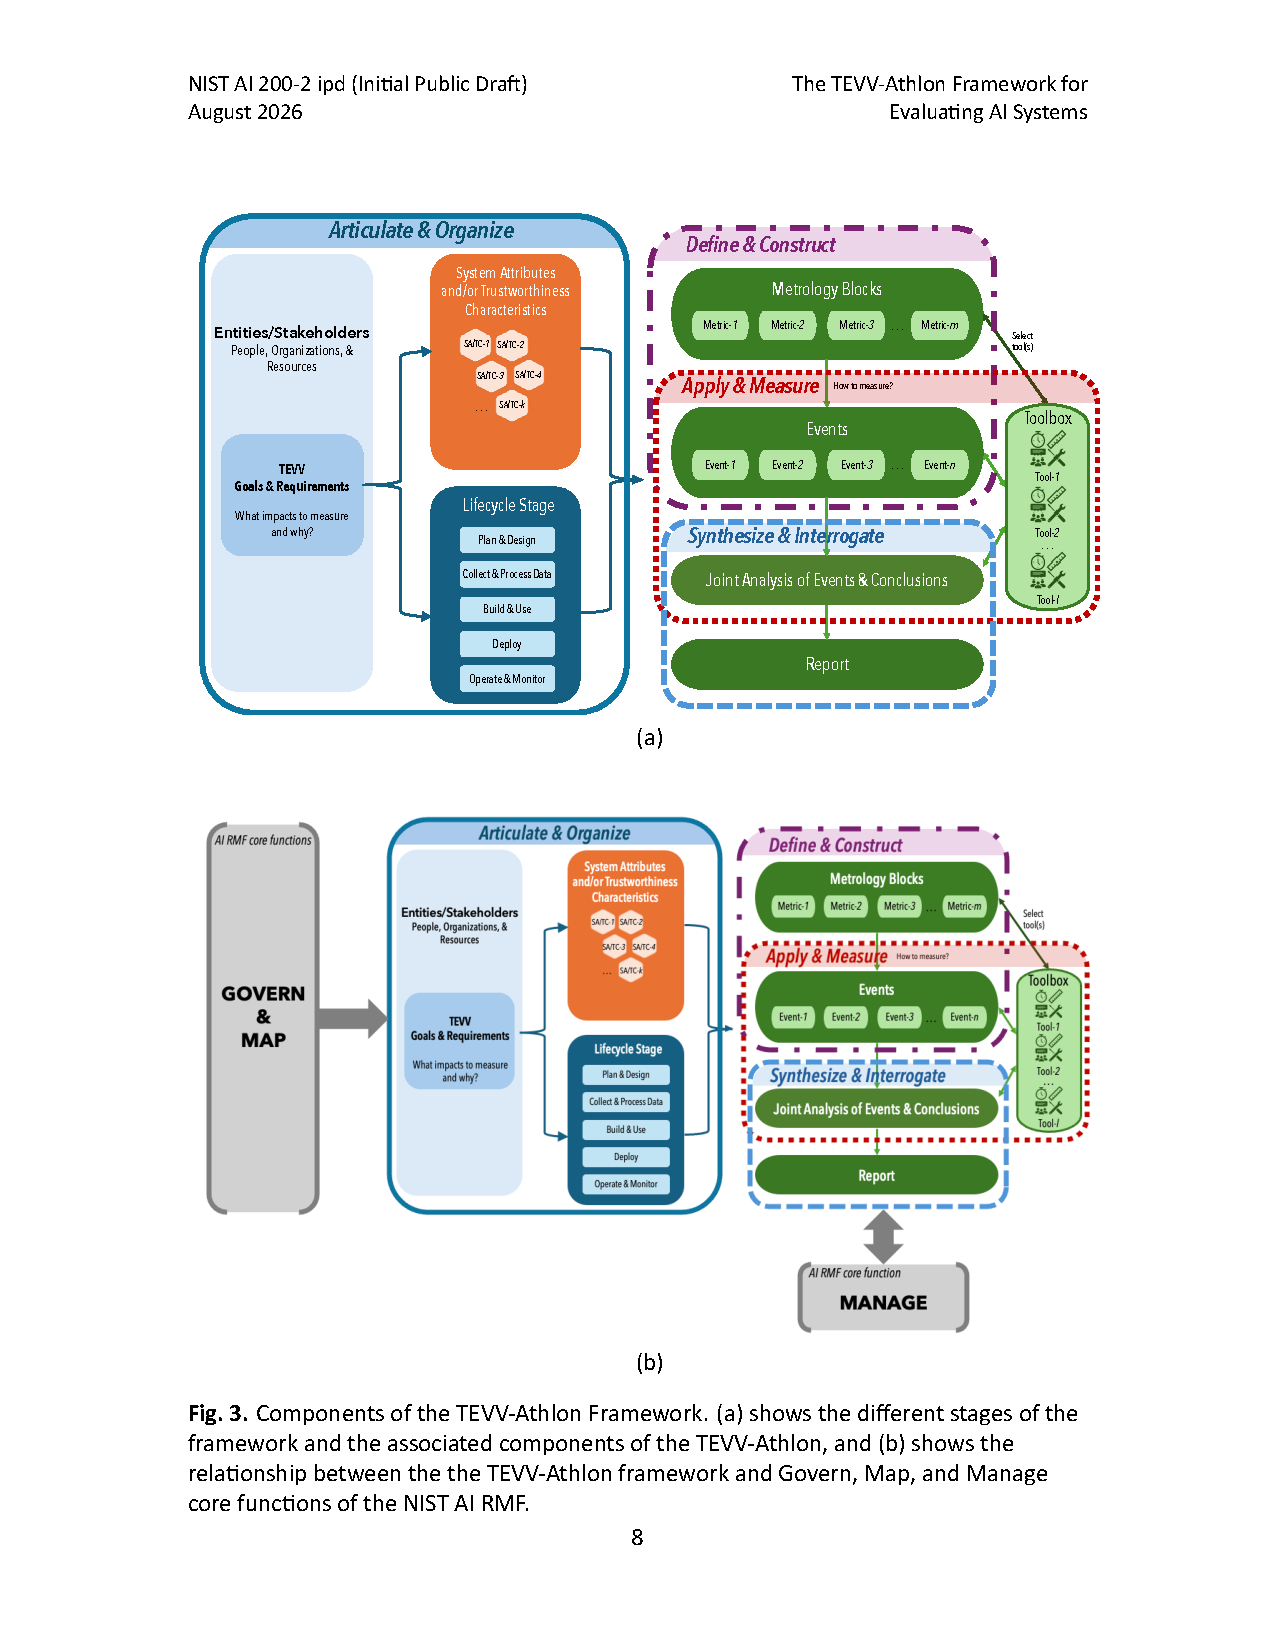
\includegraphics[width=.94\linewidth,height=.63\textheight,keepaspectratio,trim=85pt 155pt 55pt 390pt,clip]{asset/nist-ai-200-2-figure3.pdf}
\visualdescription{The TEVV-Athlon framework connects structured measurement evidence to the AI RMF Govern, Map, and Manage functions.}
\end{columns}
\slidesource{\parencite{Wallach2024EvaluatingGenerativeAi}; \parencite{Phillips2026TEVVAthlon}, \href{https://doi.org/10.6028/NIST.AI.200-2.ipd}{Figure 3(b)}}
\end{frame}

\begin{frame}{Measurement science makes TEVV claims defensible}
\footnotesize
\begin{block}{Evaluate the system and the instrument}
For LLMs, instruments include prompts, benchmark items, rubrics, raters, surveys, interview protocols, and scoring code. Their quality constrains the claims a score can support.
\end{block}
\begin{columns}[T]
\column{.48\textwidth}
\textbf{Measurement quality}
\begin{itemize}
  \item Define the objective, construct, and intended interpretation before selecting a metric.
  \item Validate that the instrument captures the intended property, covers important facets, generalizes beyond test conditions, and relates to real-world outcomes.
  \item Calibrate against baselines or ground truth; report uncertainty, variability, assumptions, and limitations.
\end{itemize}
\column{.48\textwidth}
\textbf{Experimental and process design}
\begin{itemize}
  \item Select data that reflect the intended context and prevent test-data contamination.
  \item Specify variables, conditions, procedures, and comparison points; repeat and sample to expose variation.
  \item Preserve enough detail for verification, invite independent challenge, and revalidate as systems, users, and environments change.
\end{itemize}
\end{columns}
\slidesource{\parencite{Phillips2026TEVVAthlon}, \href{https://doi.org/10.6028/NIST.AI.200-2.ipd}{Section 4.4--4.5 and Appendices D--E}}
\end{frame}

\begin{frame}{Model, adversarial, and field tests answer different questions}
\small
\begin{columns}[c]
\column{.54\textwidth}
\begin{tabularx}{\linewidth}{>{\bfseries}lY}
\toprule
Model testing & Can scripted inputs confirm claimed capabilities and guardrails?\\
Red teaming & Can motivated testers discover adverse outcomes or defeat safeguards?\\
Field testing & How do representative people use, interpret, rely on, and act on the system in context?\\
\bottomrule
\end{tabularx}
\par\vspace{.8em}
\parbox{\linewidth}{\raggedright No level dominates the others. Together they move from repeatable component evidence toward sociotechnical effects.}
\column{.42\textwidth}
\centering
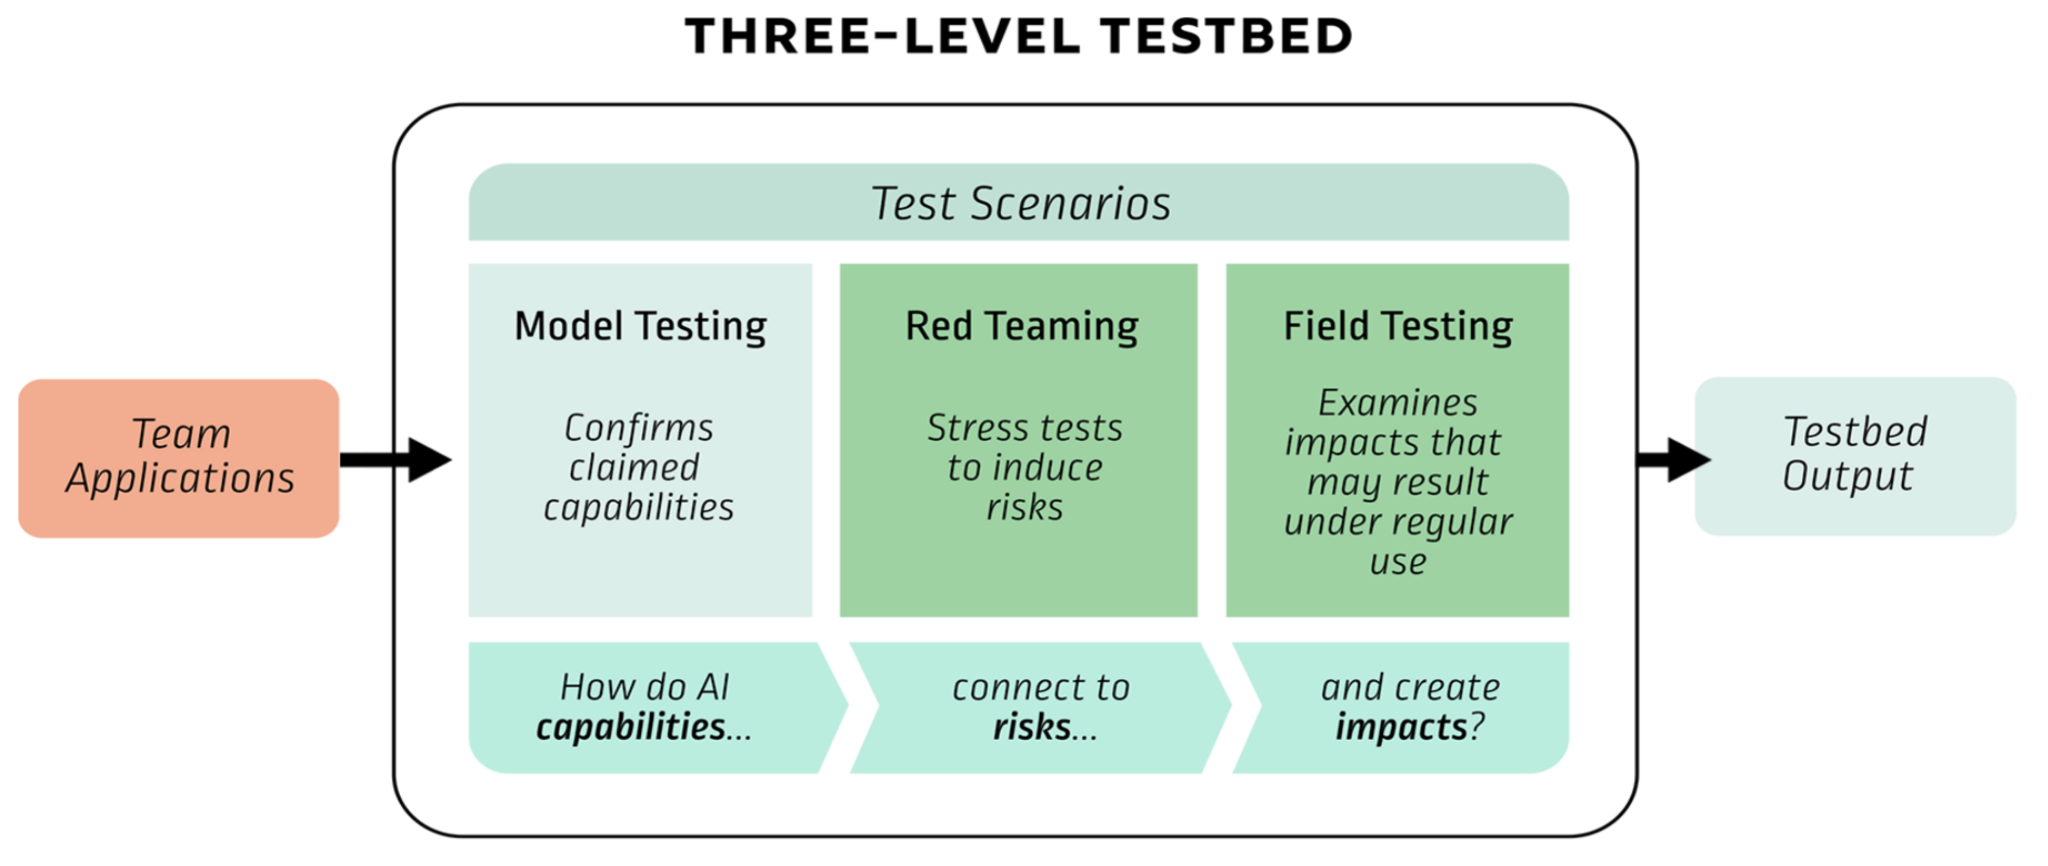
\includegraphics[width=\linewidth,height=.58\textheight,keepaspectratio]{asset/aria.jpg}
\par\vspace{.3em}
\visualdescription{ARIA connects model testing, red teaming, and field testing within one layered evaluation design.}
\end{columns}
\slidesource{\parencite{Amironesei2025AssessingRisksImpacts}, \href{https://doi.org/10.6028/NIST.AI.700-2}{ARIA 0.1 pilot evaluation}}
\end{frame}

\section{Model testing}

\begin{frame}{A benchmark is a measurement instrument}
\small
\begin{columns}[c]
\column{.49\textwidth}
\begin{block}{Benchmark specification}
\scriptsize
Population and sampling frame $\rightarrow$ task cases $\rightarrow$ prompt and decoding protocol $\rightarrow$ scorer $\rightarrow$ aggregation $\rightarrow$ claim.
\end{block}
\begin{itemize}
  \item Define the construct before selecting the dataset.
  \item Freeze versions, prompts, tools, and settings.
  \item Include baselines, negative controls, slices, and failures.
  \item Report sample size and uncertainty, not only a rank.
\end{itemize}
\column{.47\textwidth}
\centering
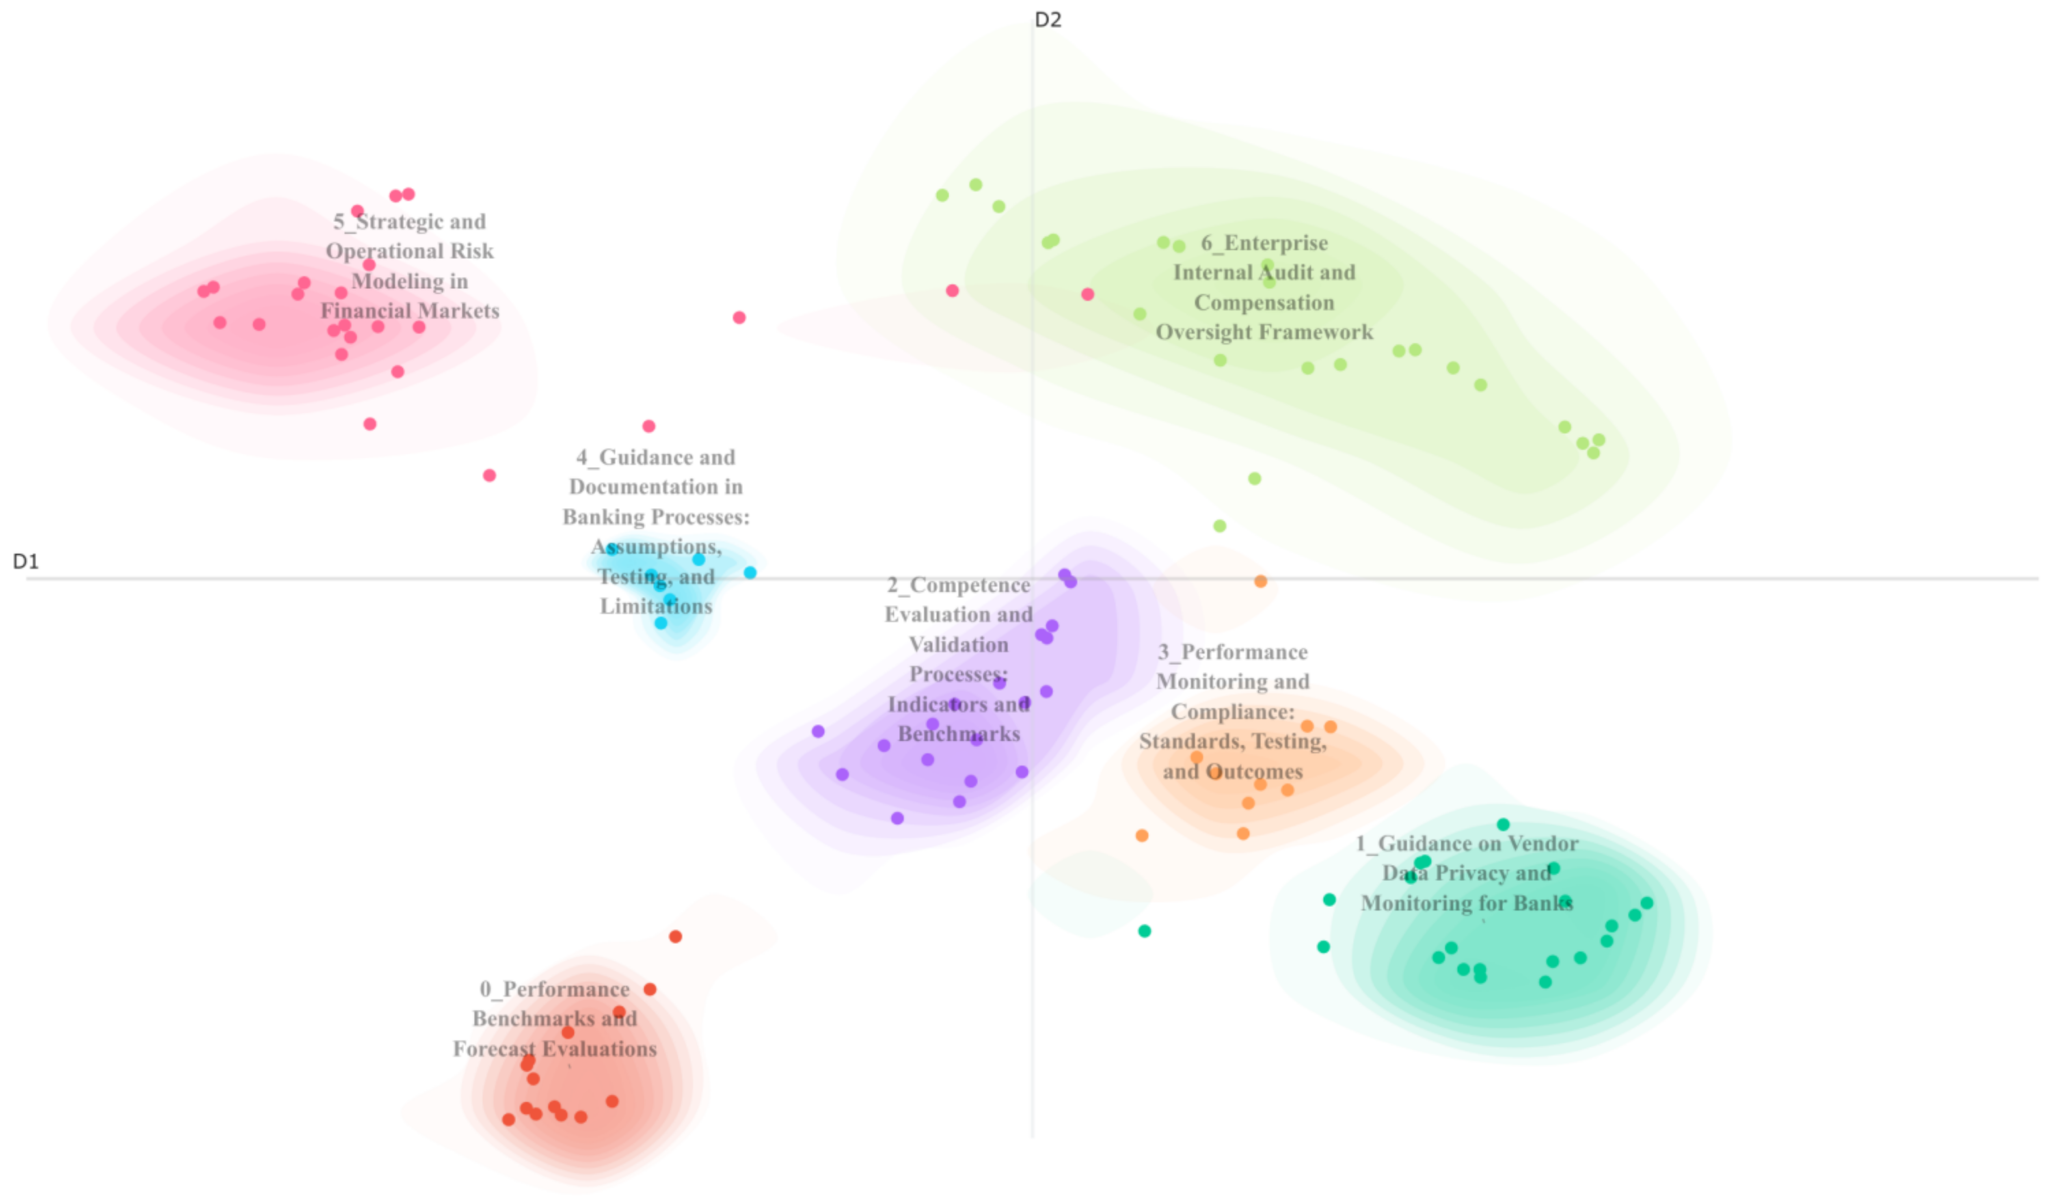
\includegraphics[width=\linewidth,height=.62\textheight,keepaspectratio]{asset/model-testing-benchmarks-and-embeddings.png}
\visualdescription{A model-testing workflow combines benchmark cases and embedding-based diagnostics rather than relying on one aggregate score.}
\end{columns}
\slidesource{\parencite{Hendrycks2021MeasuringMassiveMultitask}; \parencite{Chen2021EvaluatingLargeLanguage}; Hall, 2026, \href{https://github.com/jphall663/GWU_LLM}{\emph{AI Governance Accelerator} (GW TRAILS Institute)}}
\end{frame}

\begin{frame}{Score the task, then inspect uncertainty and slices}
\small
\begin{columns}[c]
\column{.47\textwidth}
\begingroup
\setlength{\abovedisplayskip}{.25em}
\setlength{\belowdisplayskip}{.25em}
\setlength{\abovedisplayshortskip}{.15em}
\setlength{\belowdisplayshortskip}{.15em}
For binary correctness on $n$ cases:
\[
\widehat{p}=\frac{1}{n}\sum_{i=1}^{n}\mathbb{1}(\hat y_i=y_i)
\]
\[
\operatorname{SE}(\widehat p)\approx\sqrt{\frac{\widehat p(1-\widehat p)}{n}}.
\]
\endgroup
\begin{itemize}
  \item Prefer confidence intervals or bootstrap intervals to naked point estimates.
  \item Compare paired outputs when systems see the same cases.
  \item Break results down by task, language, demographic group, difficulty, and failure mode.
\end{itemize}
\column{.49\textwidth}
\centering
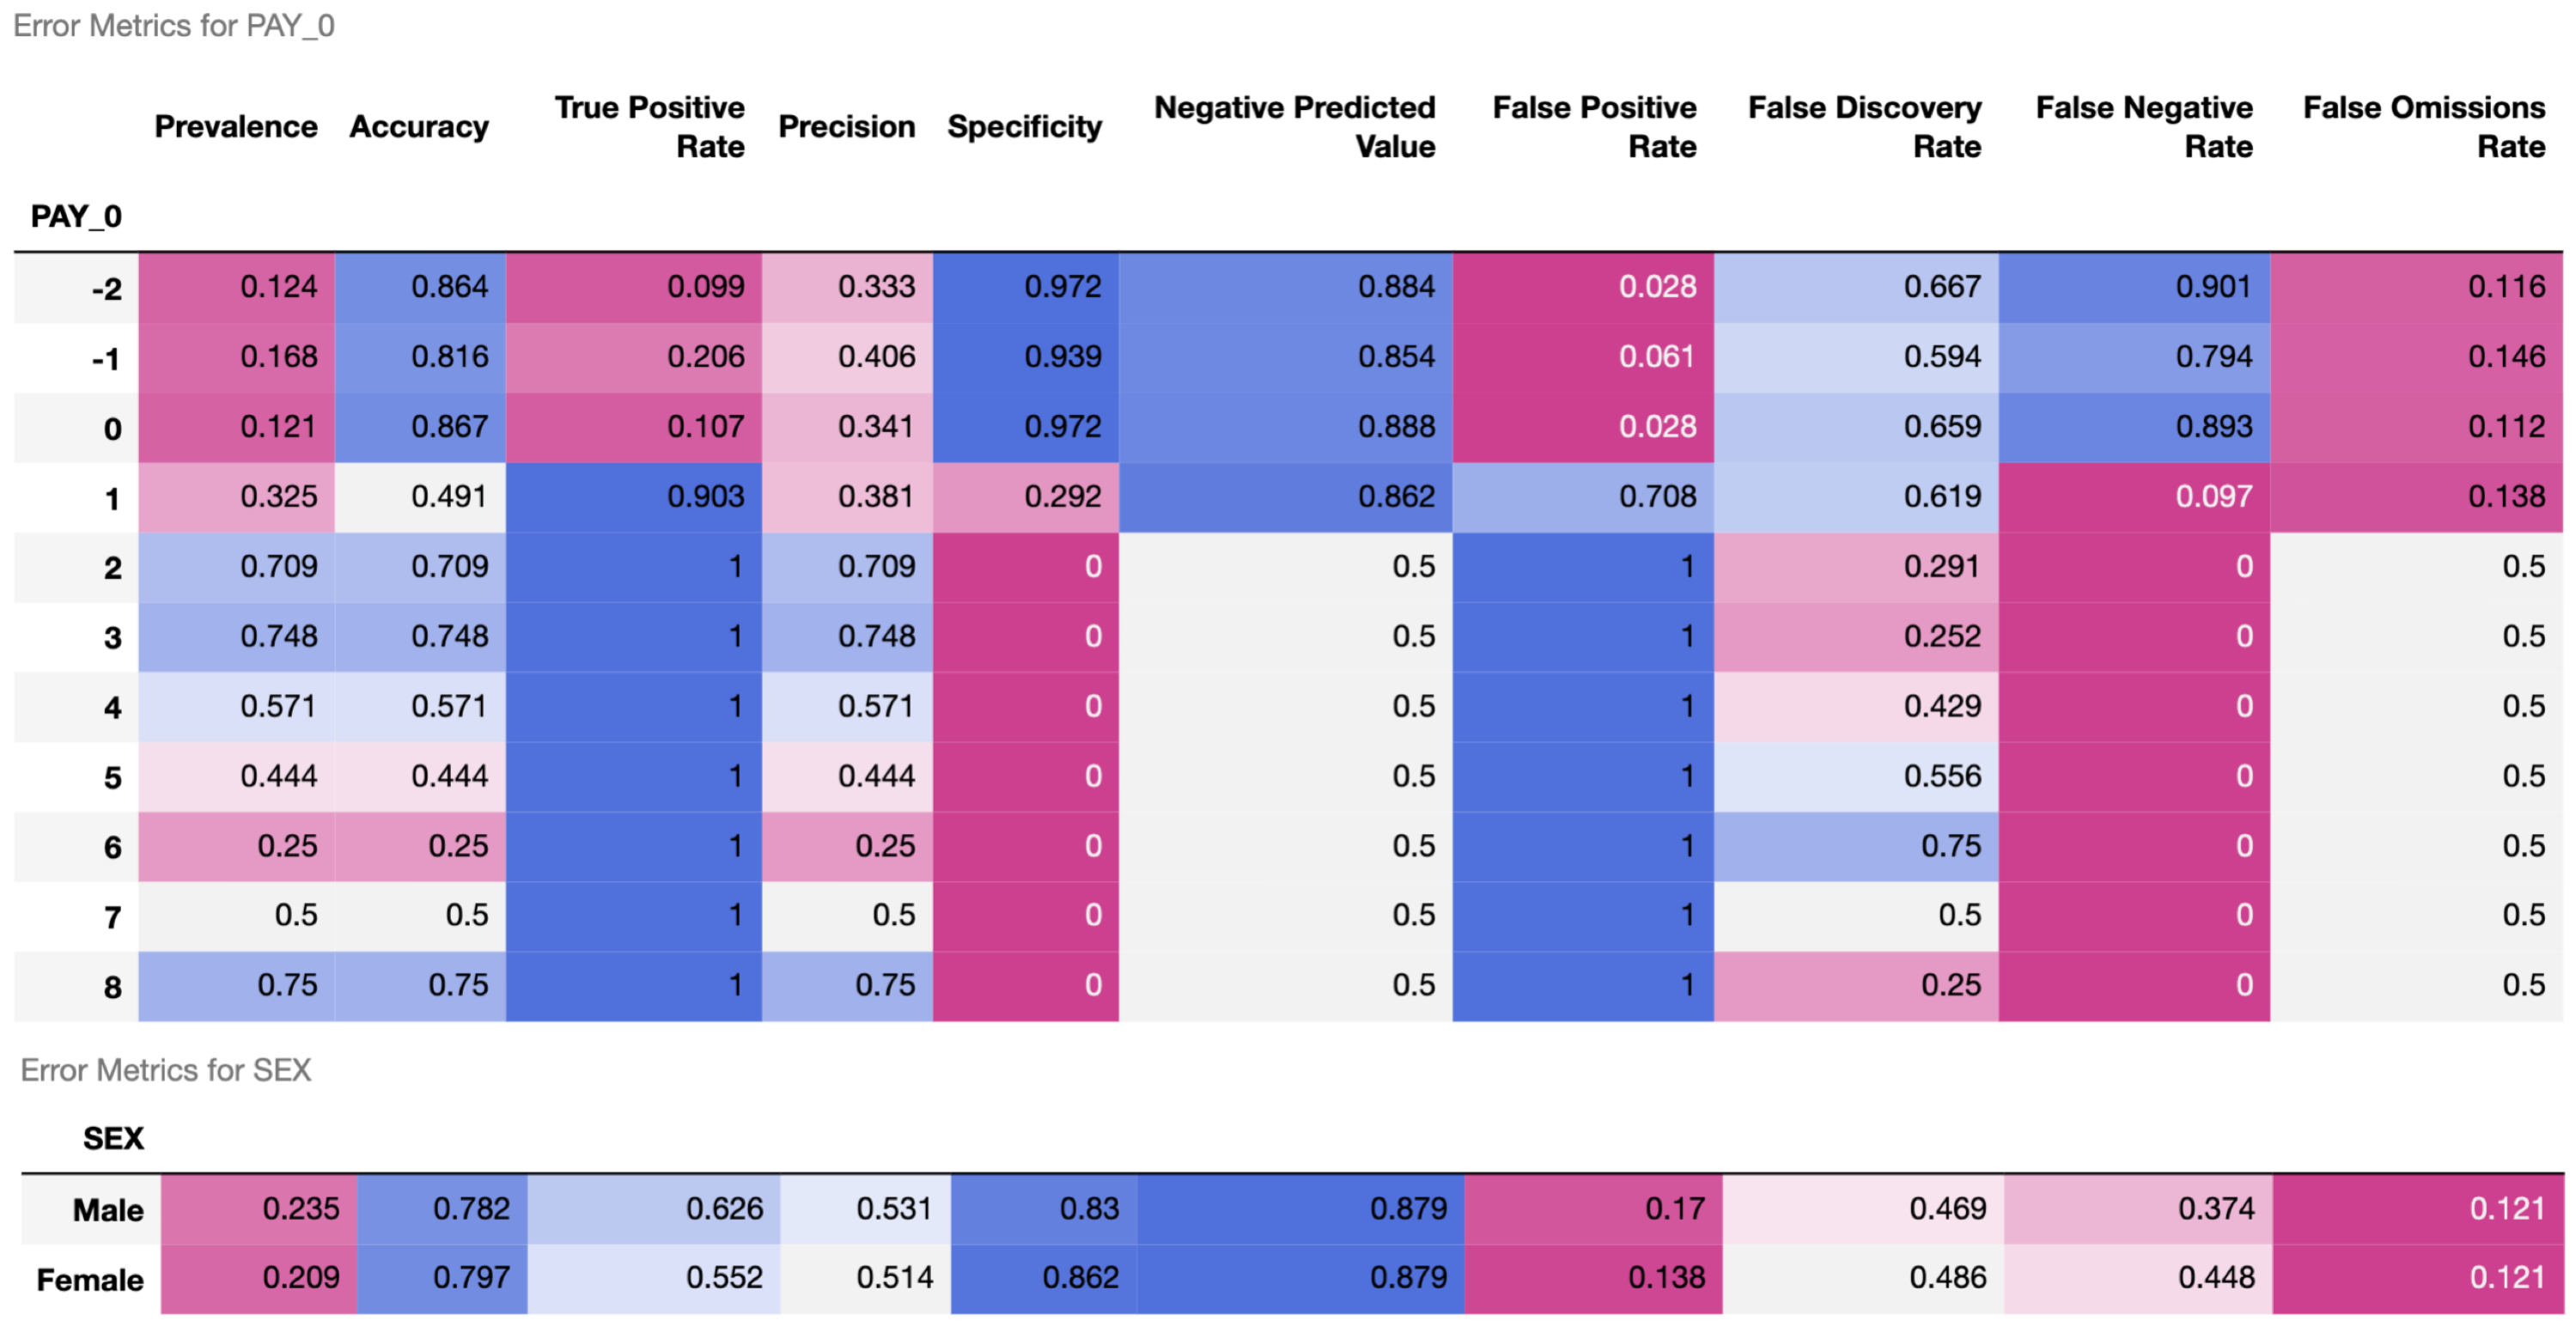
\includegraphics[width=\linewidth,height=.57\textheight,keepaspectratio]{asset/model-testing-segmented-error-analysis.png}
\visualdescription{Segmented error analysis reveals performance differences hidden by an overall average.}
\end{columns}
\slidesource{Hall, 2026, \href{https://github.com/jphall663/GWU_LLM}{\emph{AI Governance Accelerator} (GW TRAILS Institute): segmented error analysis}; \parencite{Phillips2026TEVVAthlon}}
\end{frame}

\begin{frame}{Benchmark scores can support claims they do not warrant}
\footnotesize
\begin{columns}[c]
\column{.48\textwidth}
\begin{itemize}
  \item \textbf{Construct underrepresentation}: the task covers only an easy proxy.
  \item \textbf{Contamination}: test items or near-duplicates enter development data.
  \item \textbf{Repeated reuse}: leaderboard feedback turns the test into training information.
  \item \textbf{Aggregation}: averages hide slices, variance, abstentions, and severe failures.
  \item \textbf{Staleness}: users, threats, models, and environments change.
  \item \textbf{Goodhart pressure}: optimizing the score weakens its relationship to the goal.
\end{itemize}
\column{.48\textwidth}
\centering
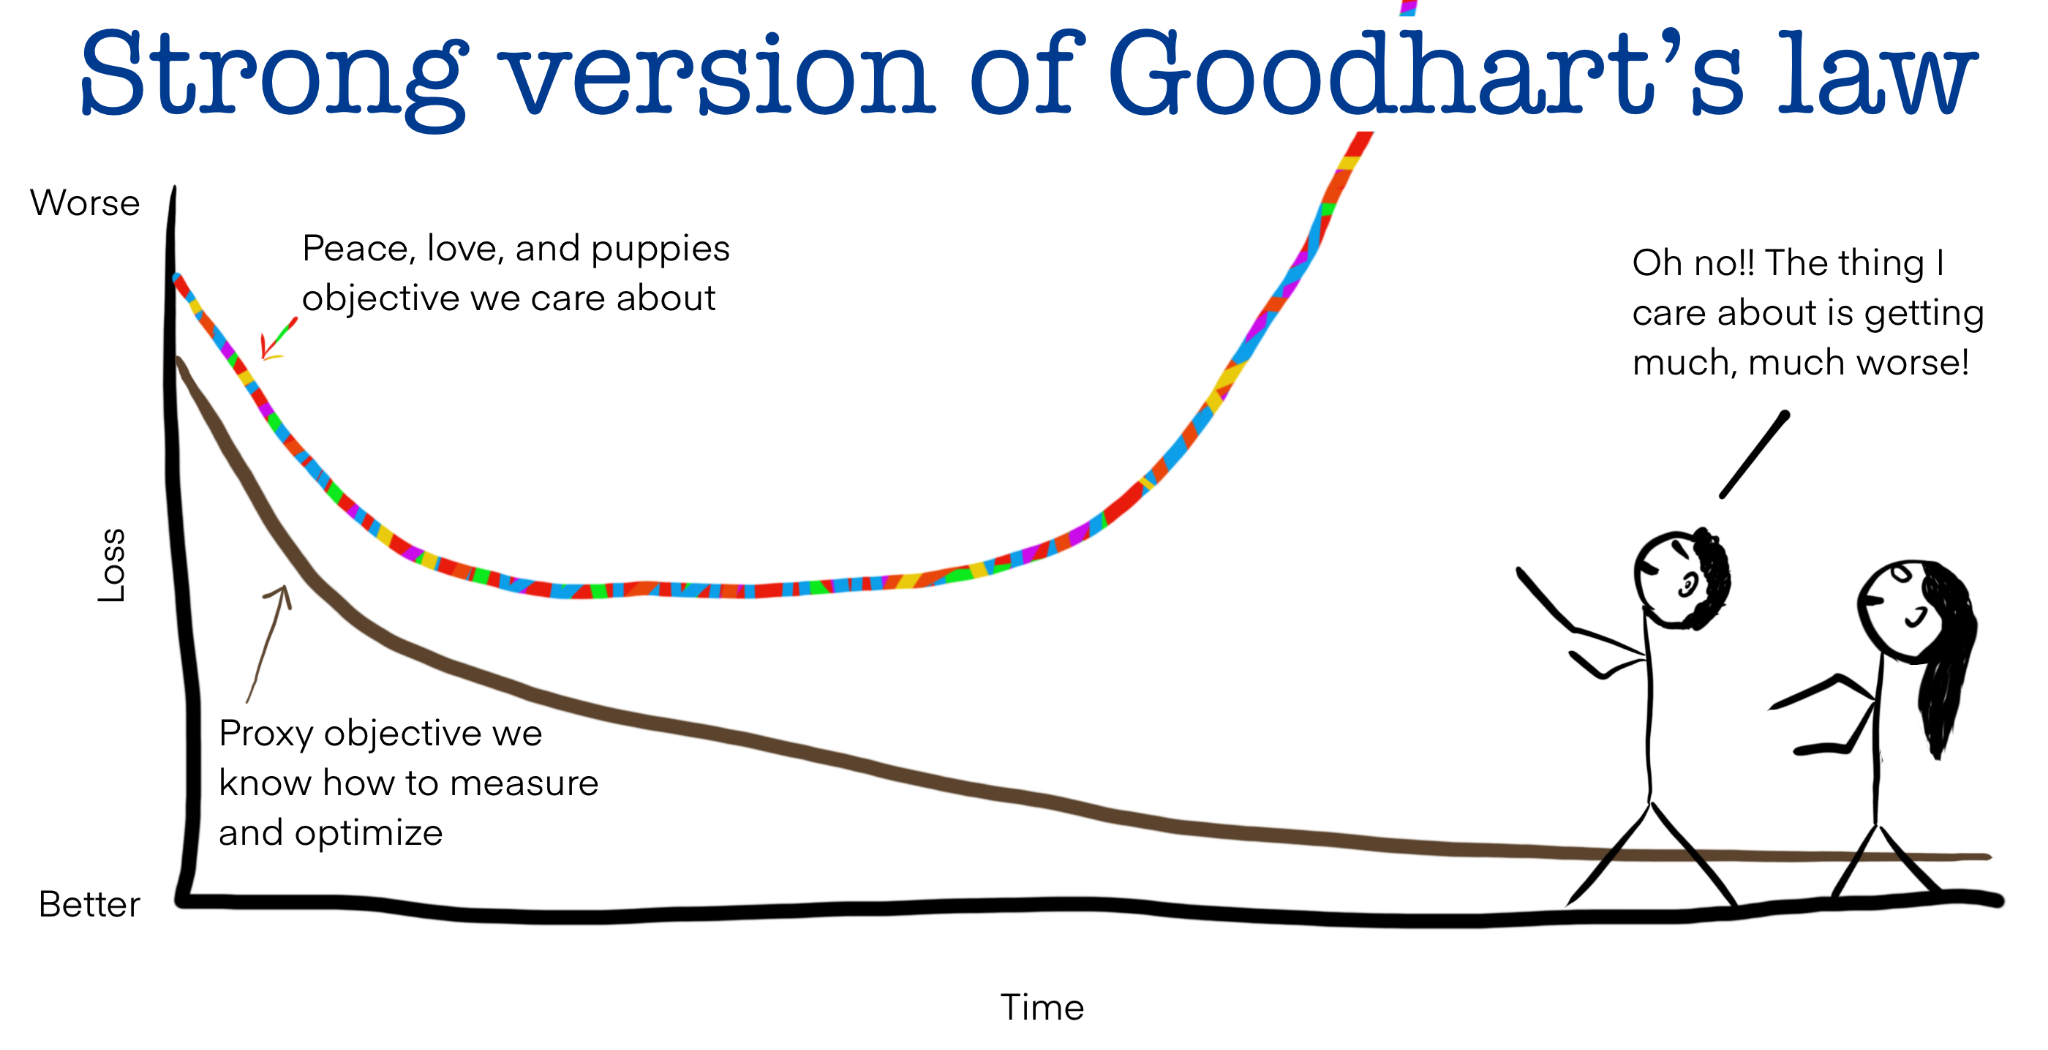
\includegraphics[width=.96\linewidth,height=.57\textheight,keepaspectratio]{asset/goodhart-law.jpg}
\visualdescription{A Goodhart's Law teaching graphic warns that a target metric may cease to represent the intended goal.}
\end{columns}
\slidesource{\parencite{Thomas2022RelianceMetricsFundamental}; \parencite{Balloccu2024LeakCheatRepeat}; Hall, 2026, \href{https://github.com/jphall663/GWU_LLM}{\emph{Guest Lecture for Prof. Pless, GW Computer Science}}}
\end{frame}

\begin{frame}{LLM-as-a-judge converts a rubric into model-mediated labels}
\footnotesize
\begin{columns}[c]
\column{.53\textwidth}
\begin{enumerate}
  \item Fix the question, reference/context, candidate answer, and rubric.
  \item Request a constrained score and concise evidence.
  \item Parse and validate the schema; keep raw outputs.
  \item Randomize answer order for pairwise judging.
  \item Repeat or use multiple judges to estimate instability.
  \item Calibrate against qualified human ratings.
\end{enumerate}
\medskip
\textbf{A judge is not ground truth:} position, verbosity, self-preference, prompt wording, and shared model failures can bias judgments.
\column{.43\textwidth}
\centering
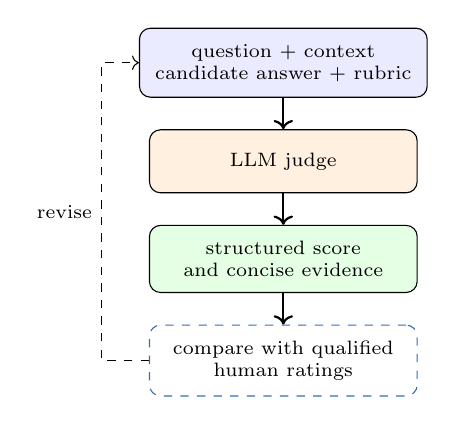
\begin{tikzpicture}[
  node distance=4mm,
  every node/.style={font=\scriptsize,align=center},
  box/.style={draw,rounded corners,minimum width=34mm,minimum height=8mm,inner sep=2mm}
]
  \node[box,fill=blue!8] (package) {question + context\\candidate answer + rubric};
  \node[box,fill=orange!12,below=of package] (judge) {LLM judge};
  \node[box,fill=green!10,below=of judge] (output) {structured score\\and concise evidence};
  \node[box,draw=brand,dashed,below=of output] (anchors) {compare with qualified\\human ratings};
  \draw[->,thick] (package)--(judge);
  \draw[->,thick] (judge)--(output);
  \draw[->,thick] (output)--(anchors);
  \draw[->,dashed] (anchors.west) -- ++(-6mm,0) |- node[pos=.25,left]{revise} (package.west);
\end{tikzpicture}
\visualdescription{An evaluation package passes through an LLM judge to produce structured scores and evidence, which are checked against qualified human ratings and used to revise the instrument.}
\end{columns}
\slidesource{\parencite{zheng2023judging}; \parencite{Liu2023GEval}; Hall, 2026, \href{https://github.com/jphall663/GWU_LLM}{\emph{Guest Lecture for Prof. Pless, GW Computer Science}}}
\end{frame}

\begin{frame}{Validate the judge as an instrument}
\scriptsize
\renewcommand{\arraystretch}{.92}
\begin{tabularx}{\textwidth}{>{\bfseries}p{.22\textwidth}Y Y}
\toprule
Signal & Test & Measurement interpretation\\
\midrule
Rubric design & Does it define and cover the target construct? & Construct/content validity\\
Process integrity & Are data, prompts, settings, parsing, and scoring correct? & Quality assurance\\
Small-change stability & Do repeated runs and irrelevant perturbations agree? & Reliability/robustness\\
Large-change sensitivity & Do construct-relevant changes move scores as expected? & Construct validity/calibration\\
Null detection & Can the judge abstain on unratable inputs? & Calibration\\
Similarity/difference & Are close cases close and meaningfully different cases separated? & Convergent/discriminant validity\\
Human agreement & Does the judge agree with qualified raters on held-out cases? & Criterion validity\\
\bottomrule
\end{tabularx}
\vspace{.25em}
\textbf{Report the instrument:} judge model/version, rubric, prompt, order policy, settings, parser, repeats, agreement, calibration sample, and known failure modes.
\slidesource{Hall, unpublished synthesis; validity and V\&V foundations \parencite{messick1987validity,cronbach1955construct,campbell1959convergent,nasa2017handbook,ieee1012-2024}; operational checks \parencite{alvarezmelis2018robustness,yeh2019infidelity,adebayo2018sanity,geifman2017selective,artstein2008intercoder,zheng2023judging}}
\end{frame}

\begin{frame}{Embeddings and classifiers test specific, bounded properties}
\small
\begin{columns}[c]
\column{.50\textwidth}
For normalized embeddings $e(x),e(y)\in\R^d$,
\[
s(x,y)=e(x)^\top e(y)
\]
can support retrieval relevance, semantic similarity, clustering, duplicate detection, and drift analysis.
\begin{itemize}
  \item A trained classifier can test toxicity, topic, policy class, or failure type at scale.
  \item Validate labels, thresholds, calibration, subgroup behavior, and domain shift.
  \item Embedding geometry is model-dependent; a two-dimensional projection is exploratory evidence.
\end{itemize}
\column{.46\textwidth}
\centering
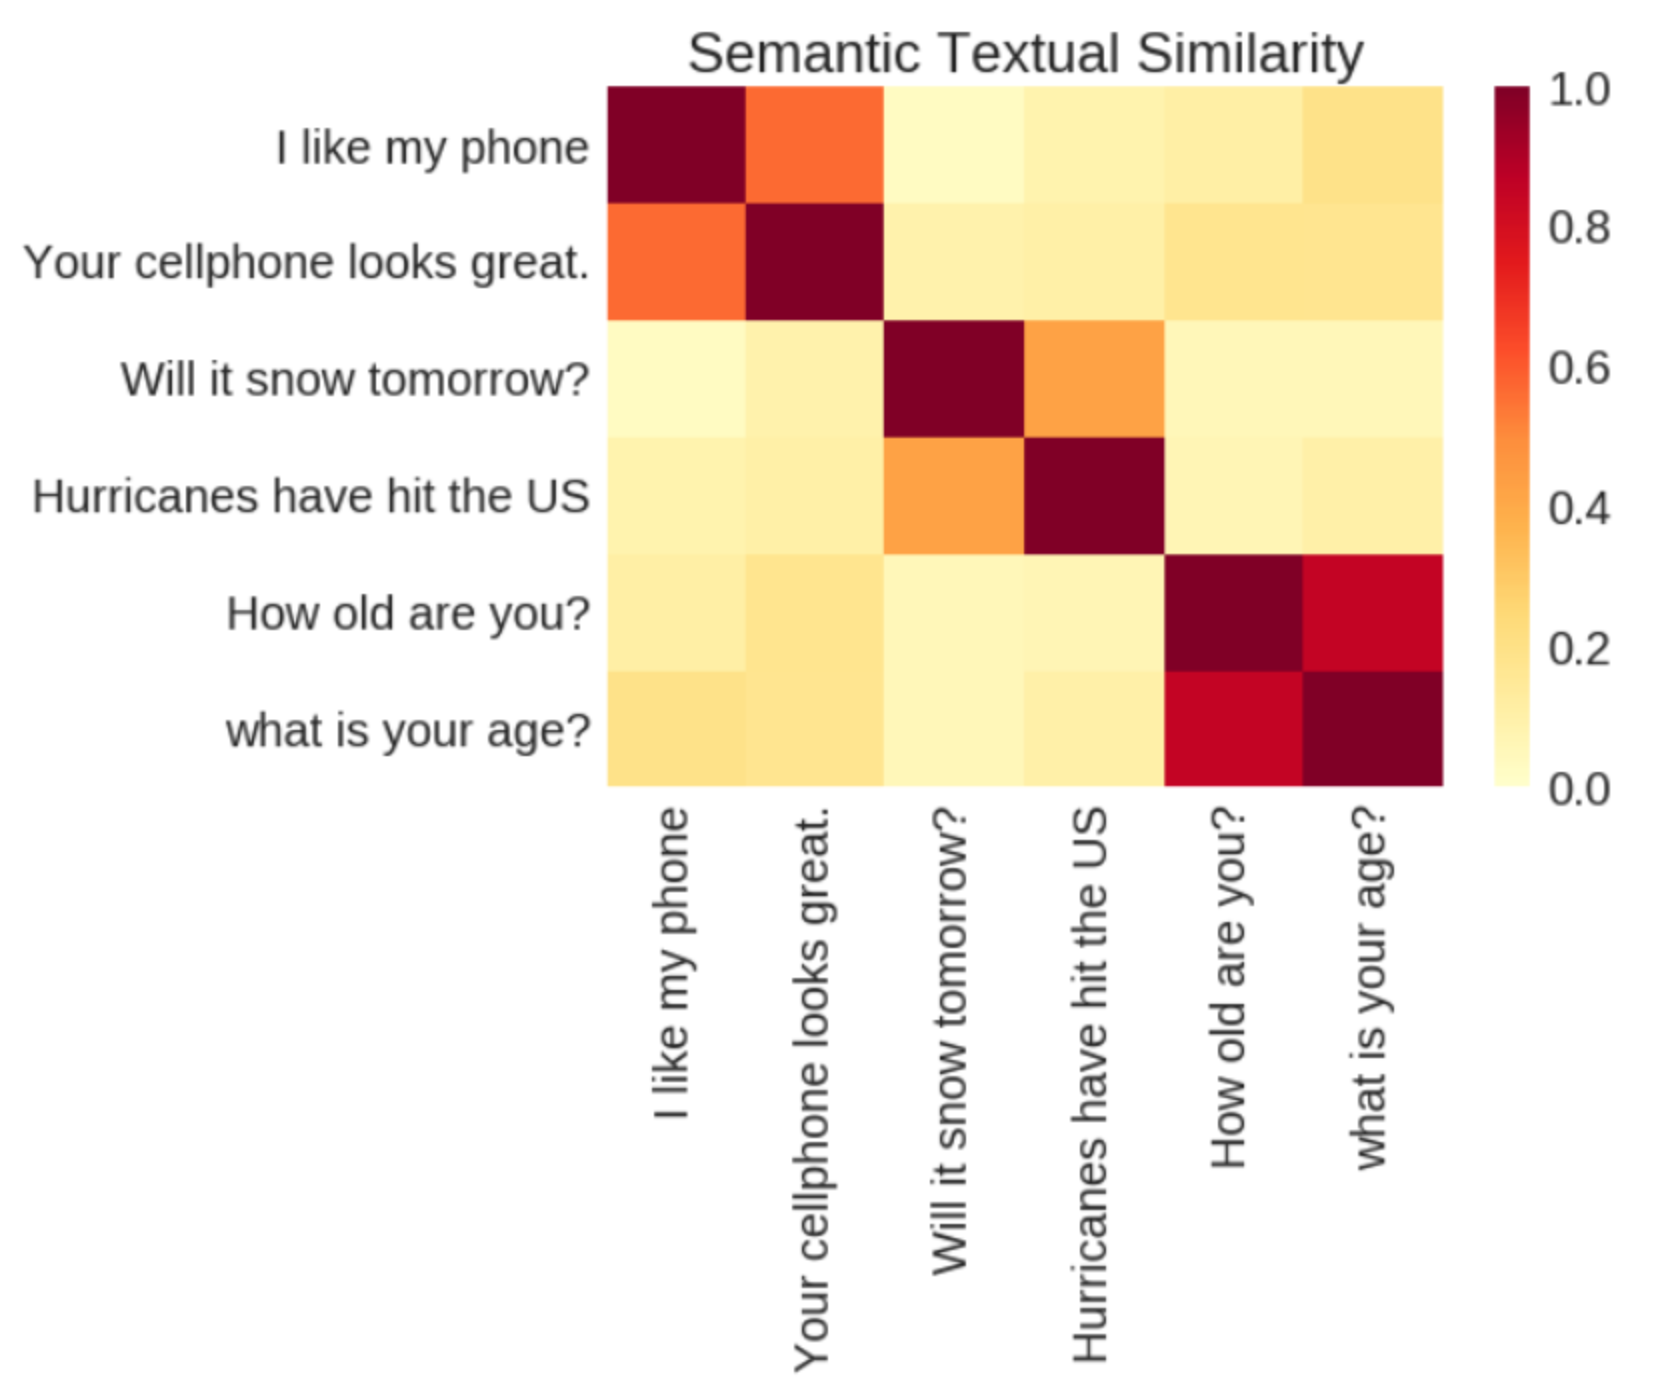
\includegraphics[width=.88\linewidth,height=.61\textheight,keepaspectratio]{asset/sentence-embeddings.png}
\visualdescription{Sentence embeddings map text into vectors whose geometry supports similarity, clustering, and classification tasks.}
\end{columns}
\slidesource{\parencite{Reimers2019SentenceBERT}; Hall, 2026, \href{https://github.com/jphall663/GWU_LLM}{\emph{AI Governance Accelerator} (GW TRAILS Institute)}}
\end{frame}

\begin{frame}{Use a battery of model tests, not one metric}
\small
\begin{columns}[c]
\column{.53\textwidth}
{\scriptsize
\renewcommand{\arraystretch}{1.08}
\begin{tabularx}{\linewidth}{>{\bfseries\raggedright\arraybackslash}p{.27\linewidth}Y}
\toprule
Method & Question\\ \midrule
Exact/schema checks & Is the output structurally and deterministically correct?\\
Reference metrics & Does it match a known answer or executable verifier?\\
Perturbation tests & Is behavior invariant to irrelevant changes?\\
Metamorphic tests & Do related inputs satisfy expected relations?\\
Slice/error analysis & Where and how does it fail?\\
Embedding tests & Does it express a bounded semantic property?\\
Repeated trials & How variable is stochastic behavior?\\
\bottomrule
\end{tabularx}
}
\column{.43\textwidth}
\centering
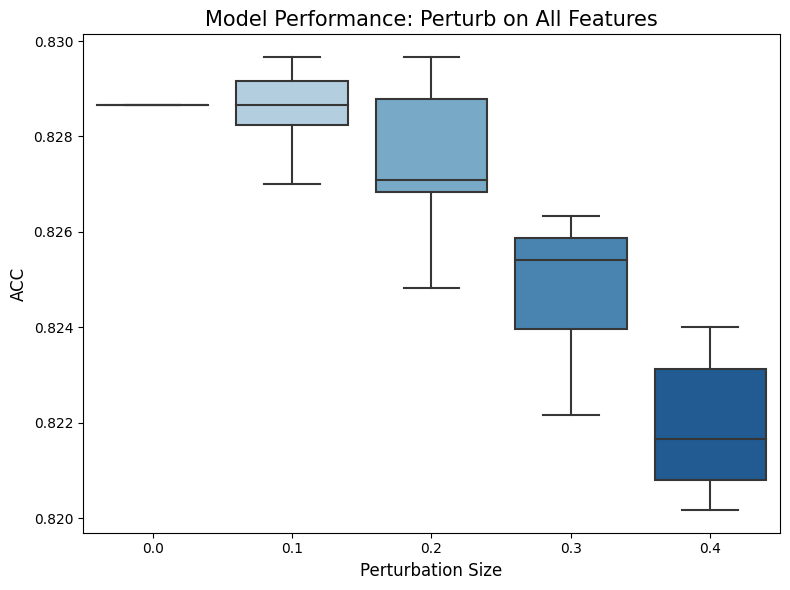
\includegraphics[width=.90\linewidth,height=.56\textheight,keepaspectratio]{asset/model-robustness-to-drift.png}
\visualdescription{A drift diagram shows data moving away from the training distribution, motivating repeated and segmented testing.}
\end{columns}
\slidesource{\parencite{Phillips2026TEVVAthlon}; Hall, 2026, \href{https://github.com/jphall663/GWU_LLM}{\emph{AI Governance Accelerator} (GW TRAILS Institute): robustness to drift}}
\end{frame}

\section{Red teaming}

\begin{frame}{Red teaming searches for consequential failures}
\small
\begin{columns}[c]
\column{.50\textwidth}
AI red teaming is a structured, authorized effort to find flaws and vulnerabilities under an adversarial mindset.
\begin{itemize}
  \item Start with assets, actors, access, harms, and system boundaries.
  \item State rules of engagement, containment, escalation, and stop conditions.
  \item Test the application, tools, retrieval layer, interface, and people---not only the base model.
  \item Record attack preconditions, transcripts, impact, reproducibility, and mitigations.
\end{itemize}
\column{.46\textwidth}
\centering
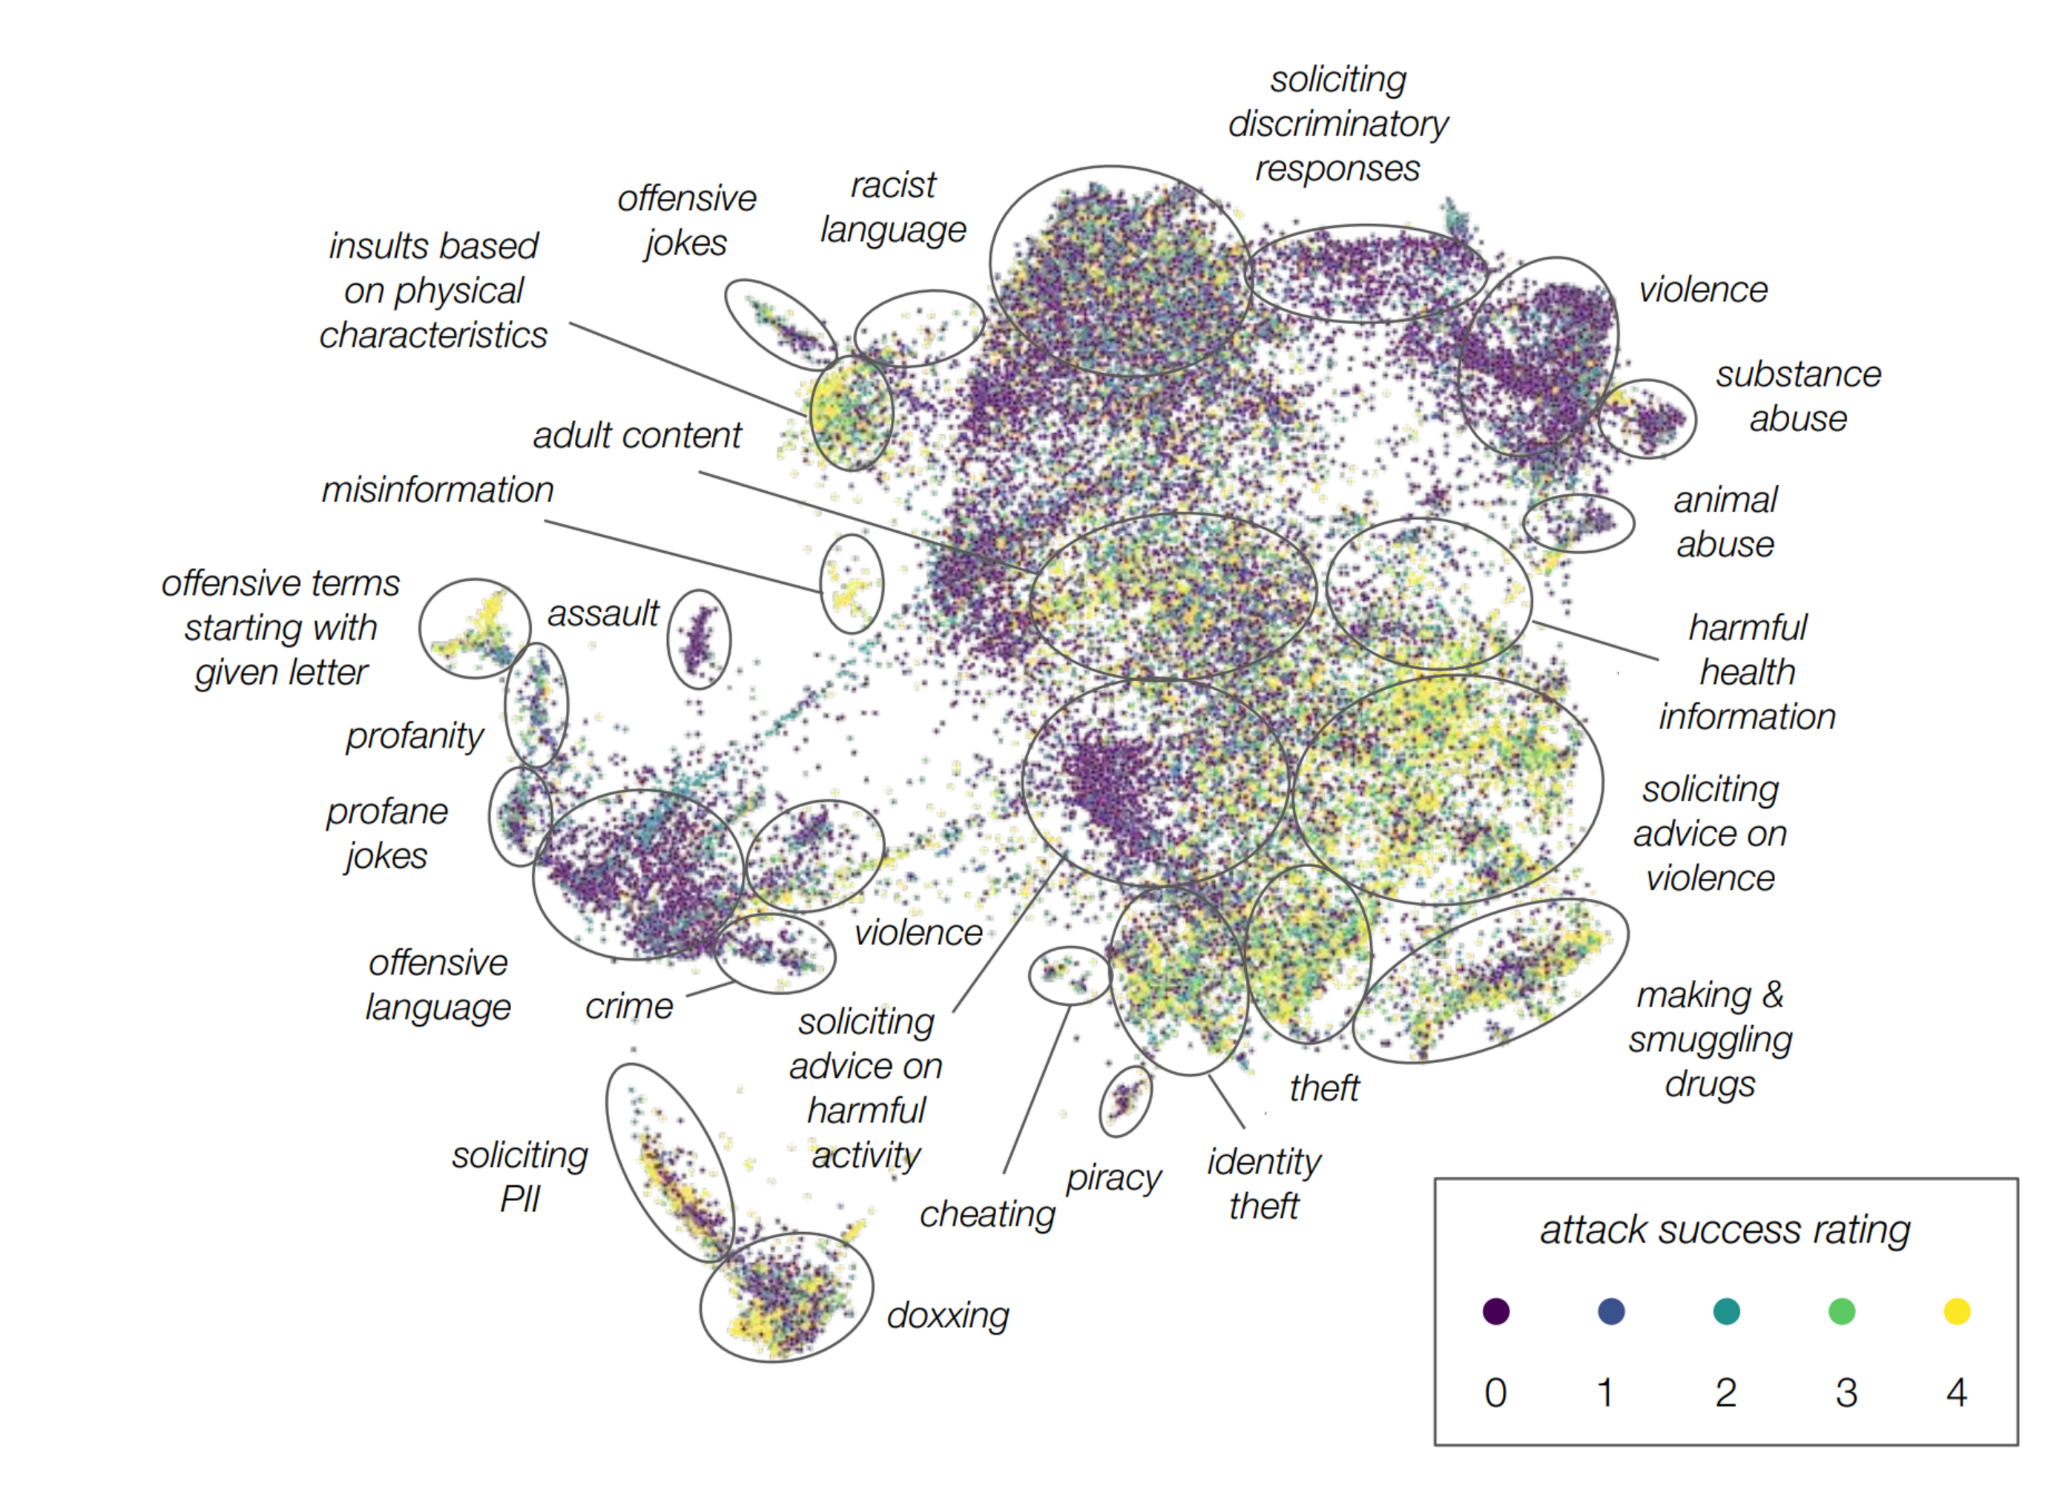
\includegraphics[width=.92\linewidth,height=.60\textheight,keepaspectratio]{asset/what-is-red-teaming.png}
\visualdescription{Anthropic clusters red-team attacks by harm type and colors them by the human tester's attack-success rating.}
\end{columns}
\vfill\tiny\color{hrgray}Source: \parencite{Perez2022RedTeamingLanguage}; \parencite{Ganguli2022RedTeamingReduceHarms}, \href{https://www-cdn.anthropic.com/files/4zrzovbb/website/82564d4ec2451b2eed2e0796b7c658fc989f0c1a.pdf}{Anthropic research memo, Figure 1.1}; Hall, 2026, \href{https://github.com/jphall663/GWU_LLM}{\emph{AI Governance Accelerator} (GW TRAILS Institute): what is red teaming?}
\end{frame}

\begin{frame}{Selected red-teaming methods}
\small
\begin{columns}[T]
\column{.48\textwidth}
\begin{block}{Security and privacy}
Test availability failures such as resource exhaustion; confidentiality failures such as prompt leakage, extraction, inversion, and membership inference; and integrity failures such as injection, poisoning, obfuscation, and retrieval manipulation.
\end{block}
\begin{block}{Fairness harms}
Hold the task constant while varying demographic groups, languages, or dialects. Counterfactual prompting tests whether comparable cases produce disparate outputs or outcomes.
\end{block}
\column{.48\textwidth}
\begin{block}{Safeguards and harmful capabilities}
Probe jailbreak susceptibility through multi-turn attacks, role-play, benign framing, or task blending; test malicious-code elicitation and unsafe use of connected tools or excessive agency.
\end{block}
\begin{block}{Factuality and knowledge robustness}
Probe expert and niche knowledge, temporal knowledge, numerical reasoning, and false premises to test whether outputs remain accurate under challenging or misleading conditions.
\end{block}
\end{columns}
\slidesource{\parencite{Phillips2026TEVVAthlon}, \href{https://doi.org/10.6028/NIST.AI.200-2.ipd}{Appendix B}; Hall, 2026, \href{https://github.com/jphall663/GWU_LLM}{\emph{AI Governance Accelerator} (GW TRAILS Institute): red-teaming methods}}
\end{frame}

\begin{frame}{Selected red-teaming methods}
\scriptsize
\renewcommand{\arraystretch}{.98}
\begin{tabularx}{\textwidth}{>{\bfseries\raggedright\arraybackslash}p{.21\textwidth}Y Y}
\toprule
Method family & Outcome under test & Example probes \\
\midrule
Availability attacks & Can service be degraded, delayed, or denied? & Sponge examples, repeated-token attacks, input overflows \\
Confidentiality attacks & Can confidential information or internal functionality be exposed? & Model extraction or inversion, membership inference, system-prompt leakage \\
Counterfactual fairness prompting & Do comparable cases receive disparate outputs or outcomes? & Hold the task fixed; vary demographic groups, languages, or dialects \\
Factuality and knowledge robustness & Do outputs remain accurate under challenging or misleading conditions? & Expert, niche, temporal, and numerical probes; false premises \\
Integrity attacks & Can inputs or data manipulate intended outputs or outcomes? & Direct or indirect injection, poisoning, obfuscation, retrieval weaknesses \\
Jailbreaking & Can prompting induce violations of safeguards? & Multi-turn or poetic attacks, benign framing, role-play, task blending \\
Malicious-code elicitation & Can the system produce exploitative or covertly harmful code? & Malware, hidden payloads, unsafe scripts, backdoored implementations \\
Agent or tool abuse & Can connected tools or external actions be misused? & Unsafe tool selection, excessive agency, unauthorized or harmful execution \\
\bottomrule
\end{tabularx}
\slidesource{Adapted from \parencite{Phillips2026TEVVAthlon}, \href{https://doi.org/10.6028/NIST.AI.200-2.ipd}{Appendix B, Table 4}}
\end{frame}

\begin{frame}{Treat a red-team campaign as an experiment}
\small
\centering
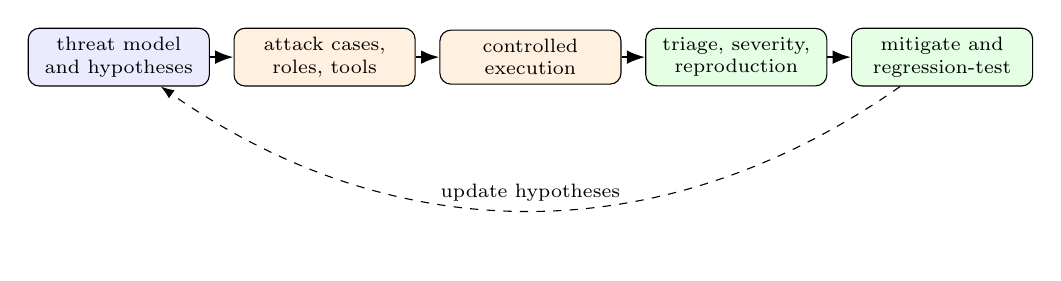
\begin{tikzpicture}[>=Latex,node distance=3mm,every node/.style={font=\scriptsize,align=center}]
\node[draw,rounded corners,fill=blue!8,minimum width=23mm] (threat) {threat model\\and hypotheses};
\node[draw,rounded corners,fill=orange!12,minimum width=23mm,right=of threat] (cases) {attack cases,\\roles, tools};
\node[draw,rounded corners,fill=orange!12,minimum width=23mm,right=of cases] (execute) {controlled\\execution};
\node[draw,rounded corners,fill=green!10,minimum width=23mm,right=of execute] (triage) {triage, severity,\\reproduction};
\node[draw,rounded corners,fill=green!10,minimum width=23mm,right=of triage] (fix) {mitigate and\\regression-test};
\draw[->,thick] (threat)--(cases); \draw[->,thick] (cases)--(execute); \draw[->,thick] (execute)--(triage); \draw[->,thick] (triage)--(fix);
\draw[->,dashed,bend left=35] (fix) to node[above]{update hypotheses} (threat);
\end{tikzpicture}
\visualdescription{A red-team campaign cycles from threat hypotheses through controlled attacks, triage, mitigation, and regression testing.}
\vspace{.8em}
\begin{columns}[T]
\column{.48\textwidth}
\begin{block}{Denominators matter}
Report success per attempt, per unique attack family, per tester, and per severity tier; include duplicate handling and tester exposure.
\end{block}
\column{.48\textwidth}
\begin{block}{Absence is bounded evidence}
``No failure found'' means no failure under the tested access, time, skills, tools, and cases---not that the system is safe.
\end{block}
\end{columns}
\slidesource{\parencite{Perez2022RedTeamingLanguage}; \parencite{NationalInstituteStandards2023ArtificialIntelligenceRisk}}
\end{frame}

\section{Field testing}

\begin{frame}{Field testing closes the context gap}
\small
\begin{columns}[c]
\column{.51\textwidth}
Field tests examine representative use in realistic settings, including the human--AI configuration and downstream actions.
\begin{itemize}
  \item Who uses the system, for which tasks, under what incentives and time pressure?
  \item What do people understand, trust, ignore, verify, or act upon?
  \item How do interfaces, policies, handoffs, and organizational controls shape outcomes?
  \item Which benefits and harms appear across groups and over time?
\end{itemize}
\column{.45\textwidth}
\centering
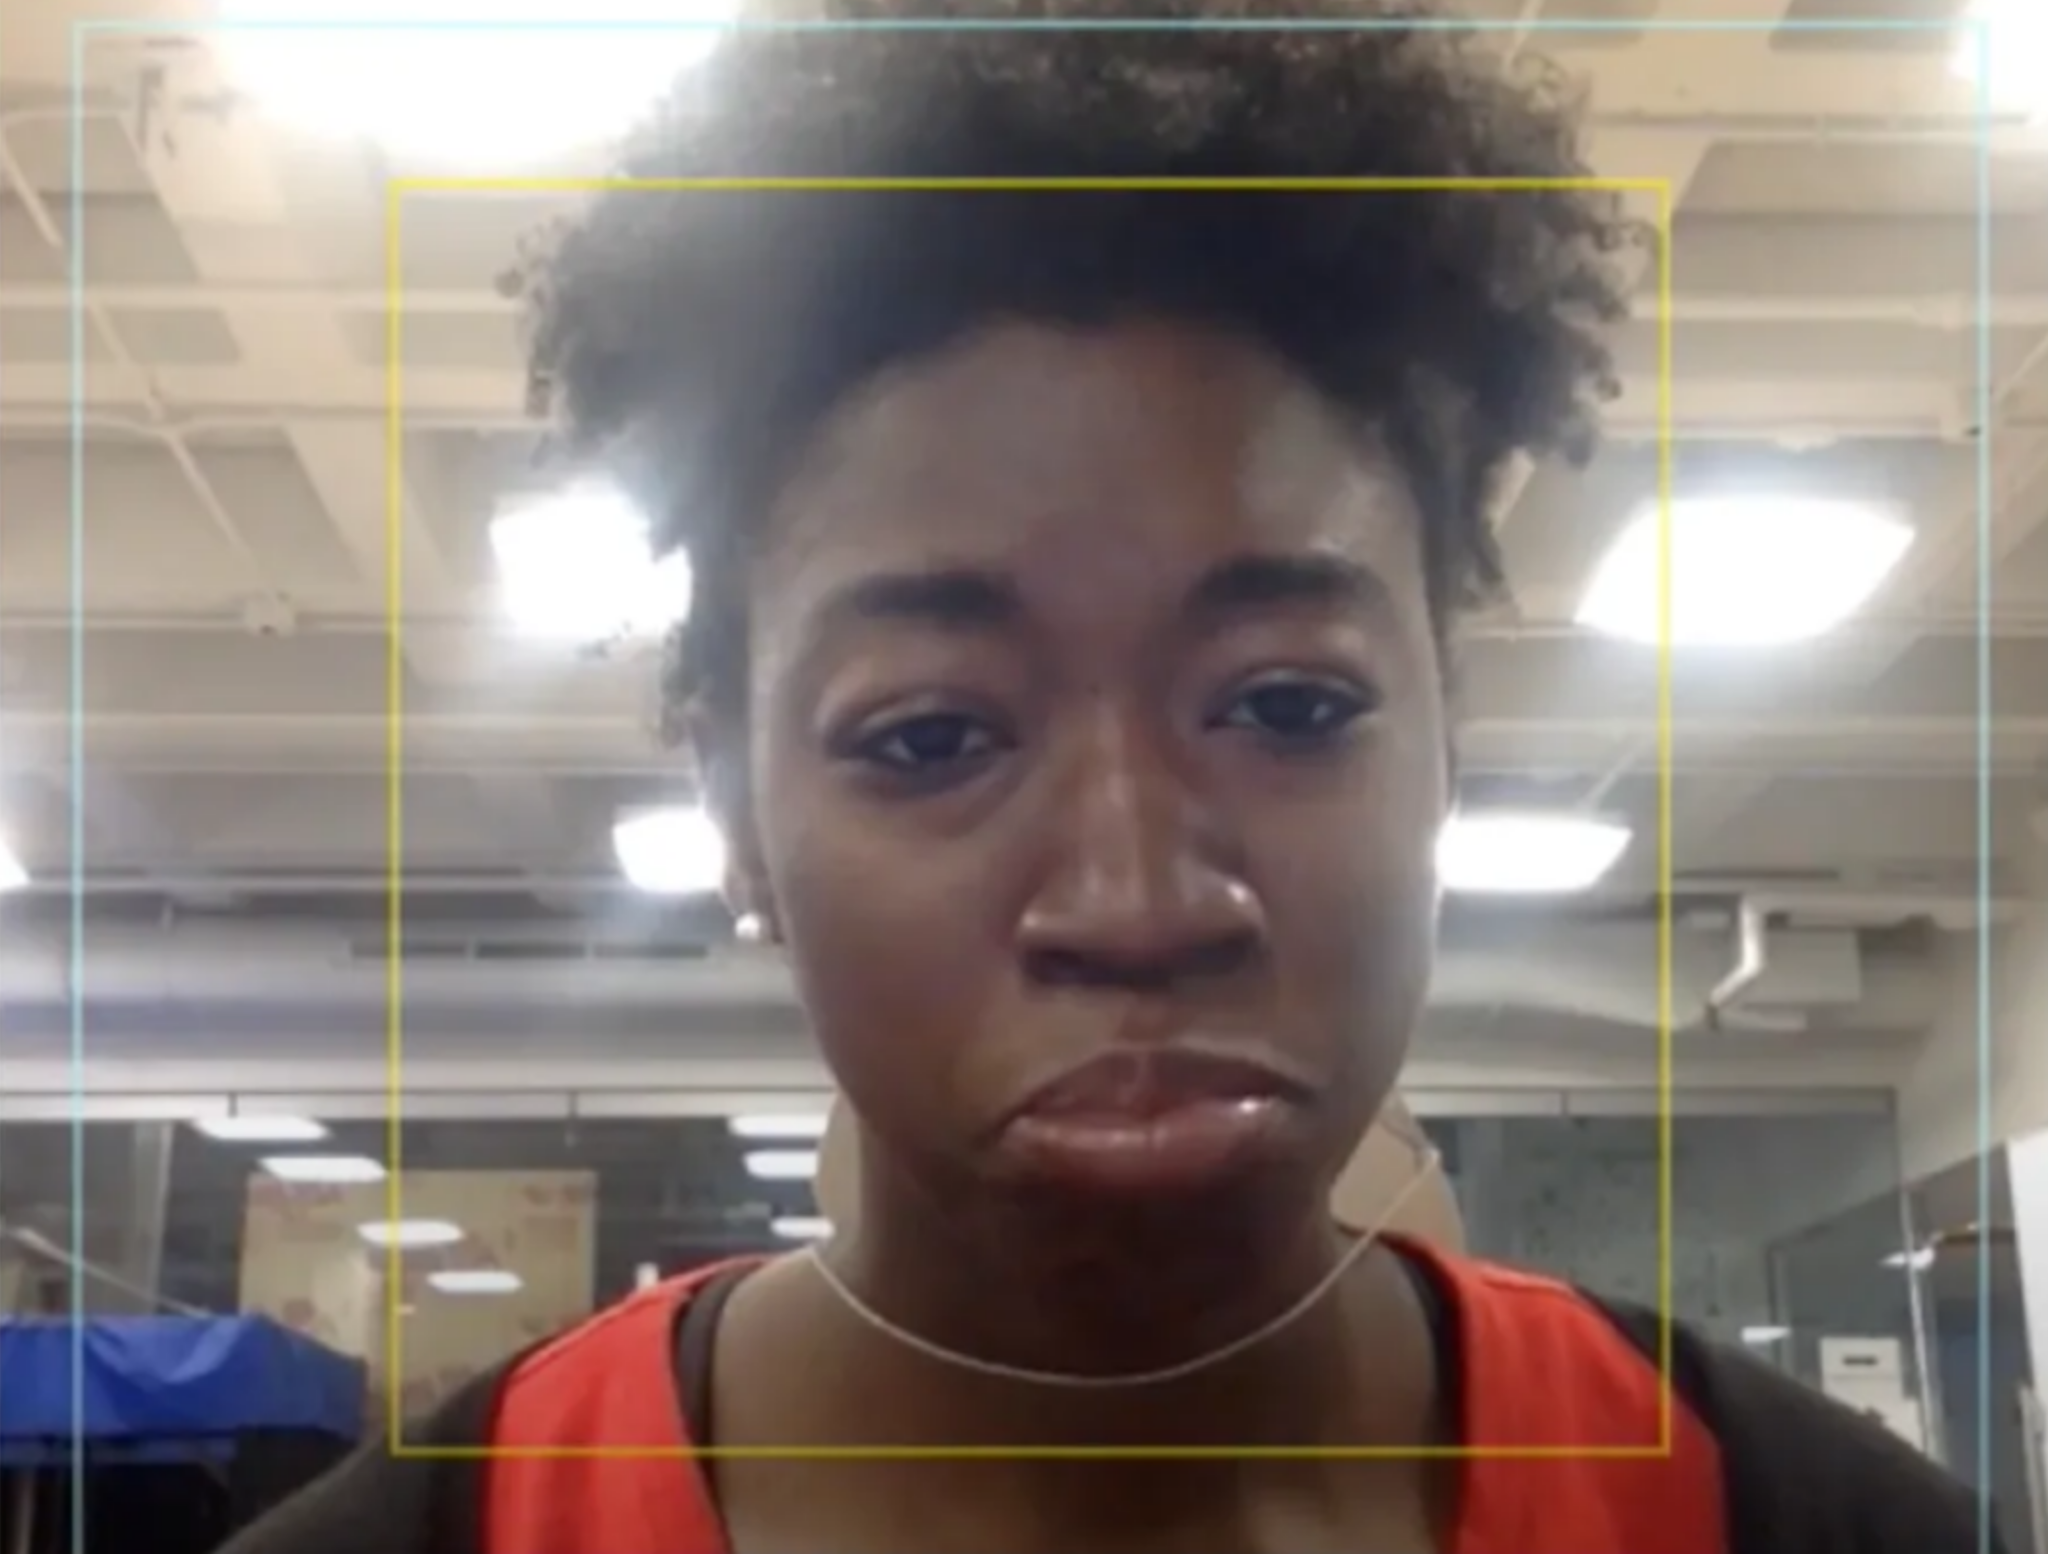
\includegraphics[width=.94\linewidth,height=.60\textheight,keepaspectratio]{asset/what-is-field-testing-1.png}
\visualdescription{Joy Buolamwini's demonstration showed a facial-analysis system failing to detect her face until she used a white mask, illustrating why field testing must include affected users and realistic conditions.}
\end{columns}
\vfill\tiny\color{hrgray}Source: Joy Buolamwini, 2016, \href{https://www.ted.com/talks/joy_buolamwini_how_i_m_fighting_bias_in_algorithms}{\emph{How I'm fighting bias in algorithms}} (video still); \parencite{Amironesei2025AssessingRisksImpacts}; \parencite{Weidinger2023SociotechnicalSafetyEvaluation}; Hall, 2026, \href{https://github.com/jphall663/GWU_LLM}{\emph{AI Governance Accelerator} (GW TRAILS Institute): what is field testing?}
\end{frame}

\begin{frame}{Selected field testing methods}
\fontsize{6.7}{7.4}\selectfont
\renewcommand{\arraystretch}{.92}
\begin{tabularx}{\textwidth}{>{\bfseries\raggedright\arraybackslash}p{.21\textwidth}Y Y}
\toprule
Method family & Outcome under test & Example evidence \\
\midrule
Impact assessment & What benefits and harms could the system create for people, organizations, and resources? & Impacts, affected groups, severity, likelihood, and mitigations \\
Field pilots & How does the system perform in a limited, realistic operational deployment? & Task outcomes, failures, workarounds, incidents, and operational constraints \\
Focus groups and interviews & How do participants understand and experience the system? & Themes, unmet needs, concerns, expectations, and contextual detail \\
Structured human-subject experiments & How does the system change human behavior, decisions, or outcomes under controlled conditions? & Comparisons across conditions, behavioral measures, and subgroup effects \\
Post-deployment feedback & Which benefits, failures, and harms emerge after release? & Ratings, complaints, support records, incident reports, and usage patterns \\
Usability and UX research & Can intended users interact with the system effectively, efficiently, and satisfactorily? & Task completion, errors, time on task, comprehension, and satisfaction \\
User surveys & What standardized perceptions and experiences do users or stakeholders report? & Scaled responses, distributions, open-text feedback, and subgroup comparisons \\
\bottomrule
\end{tabularx}
\slidesource{Adapted from \parencite{Phillips2026TEVVAthlon}, \href{https://doi.org/10.6028/NIST.AI.200-2.ipd}{Appendix C, Table 5}}
\end{frame}

\begin{frame}{Example field-testing rubric}
\scriptsize
\begin{tabularx}{\textwidth}{>{\bfseries}p{.18\textwidth}YYY}
\toprule
Dimension & 1 point & 2 points & 3 points\\ \midrule
Accuracy & Incorrect or misleading & Mostly correct; minor issues & Correct and well-qualified\\
Relevance & Off-topic & Partly responsive & Directly responsive\\
Completeness & Major omissions & Covers basics & Covers all key parts\\
Clarity & Confusing & Understandable & Clear and well organized\\
Instructions & Misses key instructions & Mostly follows & Fully follows\\
Usefulness & Not helpful & Somewhat helpful & Practical and helpful\\
Safety / fit & Unsafe or inappropriate & Generally safe; minor concerns & Safe and appropriate\\
\bottomrule
\end{tabularx}
\vspace{.45em}
\begin{columns}[T]
\column{.59\textwidth}
\textbf{Checklist:} realistic scenarios; 30--50 ratings per use case for analysis; at least three raters for agreement; repeated key questions for response variance; per-dimension review; avoid redundant dimensions and floor/ceiling effects.
\column{.37\textwidth}
\begin{block}{Interpretation}
18--21: strong\\13--17: weak\\7--12: unacceptable
\end{block}
\end{columns}
\slidesource{Hall, 2026, \href{https://github.com/jphall663/GWU_LLM}{\emph{Field Testing Rubric}}, CC BY-NC-SA 4.0}
\end{frame}

\begin{frame}{Design field evidence with people, not around them}
\footnotesize
\begin{columns}[c]
\column{.52\textwidth}
\begin{itemize}
  \item Recruit participants that reflect intended users and affected groups.
  \item Randomize or counterbalance order; define comparison conditions.
  \item Capture task success, time, reliance, overrides, confidence, comprehension, and downstream actions.
  \item Analyze participant, rater, scenario, and run-level variation.
  \item Plan consent, privacy, compensation, accessibility, deception, debriefing, and escalation.
  \item Use institutional human-subjects review when the activity is research involving people.
\end{itemize}
\column{.44\textwidth}
\centering
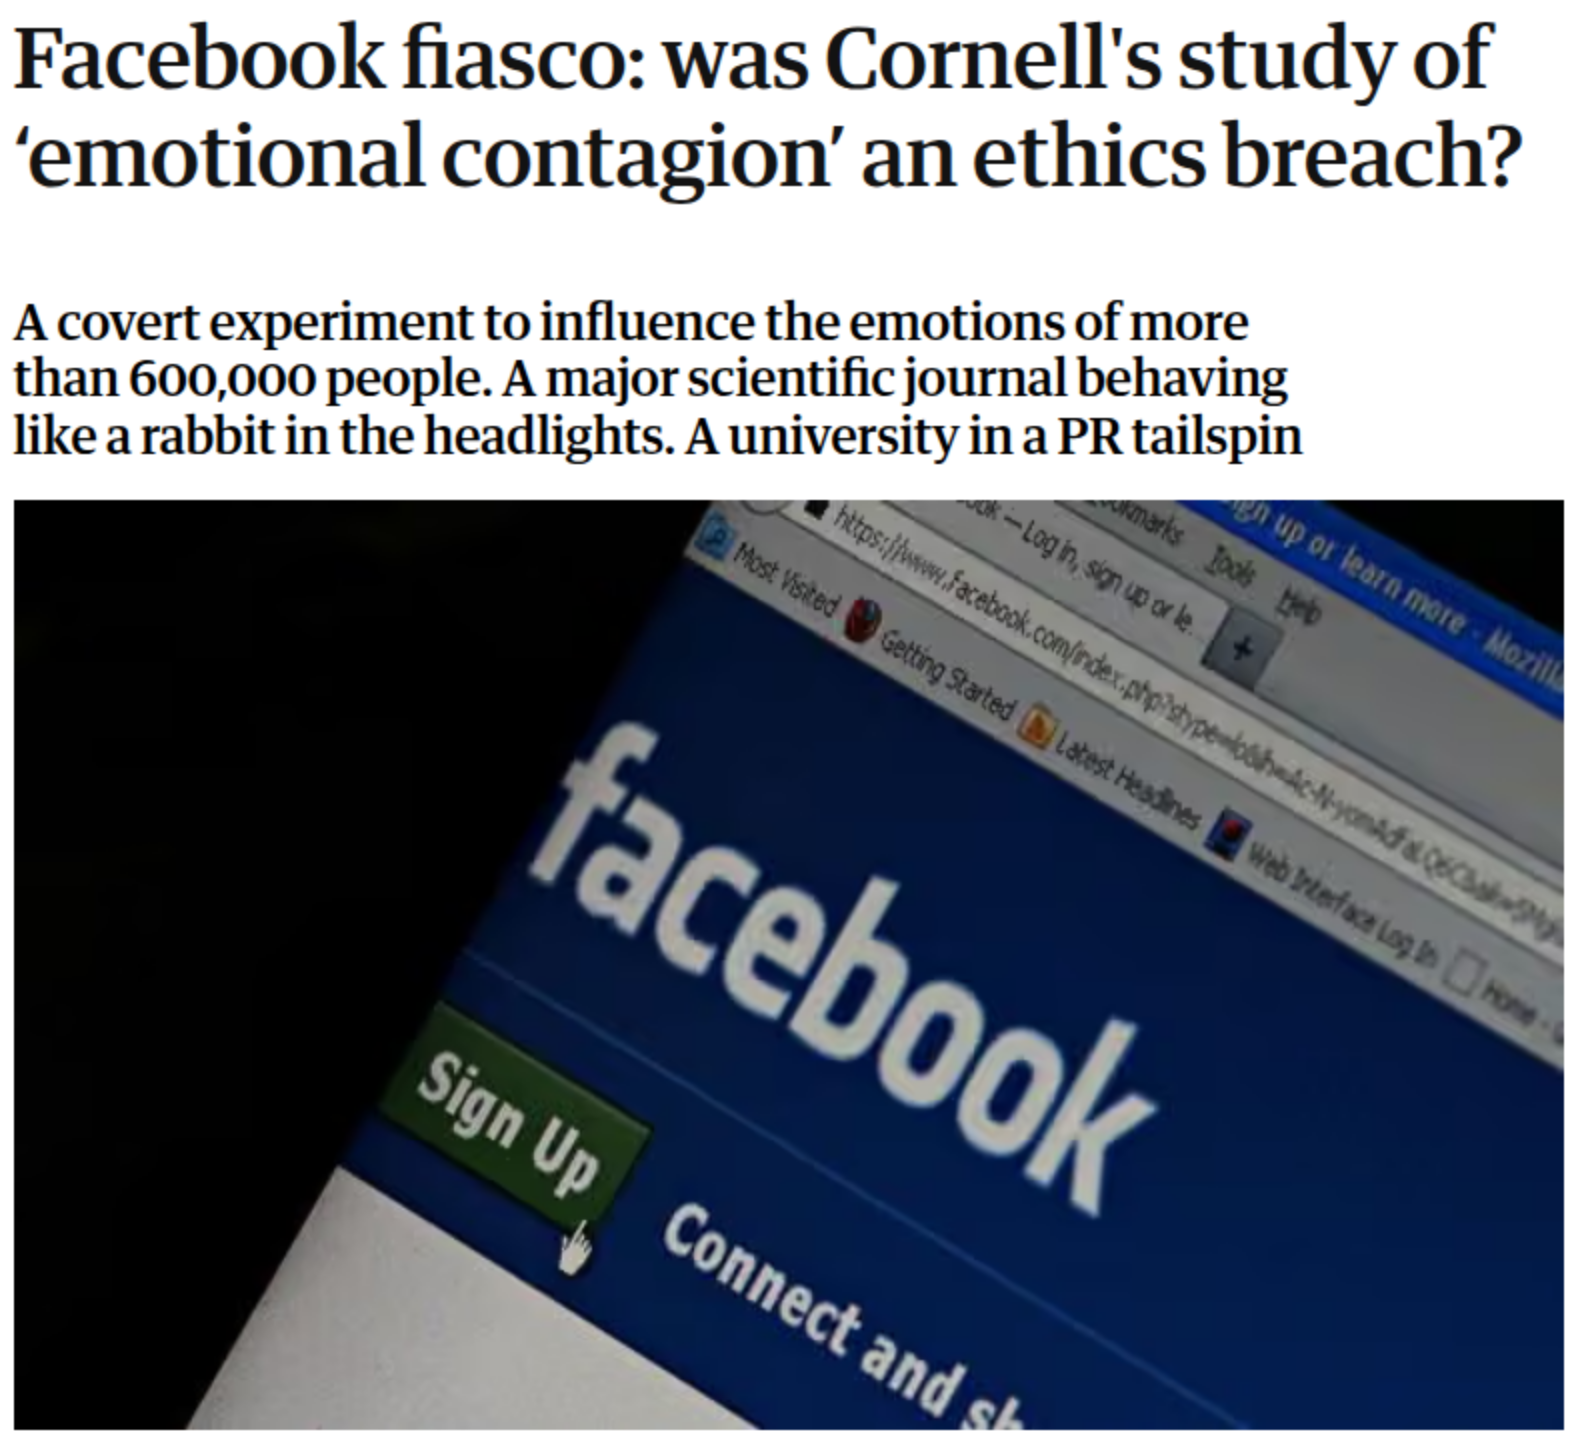
\includegraphics[width=.84\linewidth,height=.52\textheight,keepaspectratio]{asset/basics-of-human-subjects-research.png}
\visualdescription{In 2012, Facebook altered users' News Feeds to test emotional contagion without obtaining informed consent, prompting a major research-ethics controversy.}
\end{columns}
\slidesource{Chris Chambers, 2014, \href{https://www.theguardian.com/science/head-quarters/2014/jul/01/facebook-cornell-study-emotional-contagion-ethics-breach}{\emph{Facebook fiasco: was Cornell's study of ``emotional contagion'' an ethics breach?}}, \emph{The Guardian}; \parencite{Amironesei2025AssessingRisksImpacts}; Hall, 2026, \href{https://github.com/jphall663/GWU_LLM}{\emph{AI Governance Accelerator} (GW TRAILS Institute): human-subjects research}}
\end{frame}

\section{Validation and synthesis}

\begin{frame}{Synthesize evidence without hiding disagreement}
\footnotesize
\begin{columns}[T]
\column{.49\textwidth}
\small
\begin{enumerate}
  \item Map each claim to model, red-team, field, process, and monitoring evidence.
  \item Preserve separate results before aggregation.
  \item Weight evidence by relevance, quality, independence, and uncertainty.
  \item Record contradictions and missing branches explicitly.
  \item Tie acceptance criteria to a decision: deploy, deploy with conditions, defer, or reject.
\end{enumerate}
\column{.47\textwidth}
\footnotesize
\centering
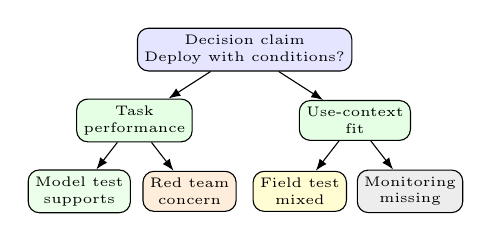
\begin{tikzpicture}[
  level distance=9mm,
  level 1/.style={sibling distance=28mm},
  level 2/.style={sibling distance=14mm},
  every node/.style={draw,rounded corners,align=center,font=\tiny,inner sep=2.5pt},
  edge from parent/.style={draw,-{Latex[length=1.5mm]}}
]
\node[fill=blue!10] {Decision claim\\Deploy with conditions?}
  child {node[fill=green!10] {Task\\performance}
    child {node[fill=green!8] {Model test\\supports}}
    child {node[fill=orange!14] {Red team\\concern}}}
  child {node[fill=green!10] {Use-context\\fit}
    child {node[fill=yellow!18] {Field test\\mixed}}
    child {node[fill=gray!14] {Monitoring\\missing}}};
\end{tikzpicture}
\visualdescription{A measurement tree keeps supporting, concerning, mixed, and missing evidence on separate branches below decision-relevant constructs.}
\begin{block}{Measurement tree}
Leaves are observed indicators; intermediate nodes are constructs; the root is the decision-level claim. Aggregation rules must be transparent and contestable.
\end{block}
\centering\scriptsize
\href{https://nvlpubs.nist.gov/nistpubs/ai/NIST.AI.700-2.pdf}{See NIST AI 700-2 for applied measurement trees.}
\end{columns}
\slidesource{\parencite{Amironesei2025AssessingRisksImpacts}; \parencite{Phillips2026TEVVAthlon}; Hall, 2026, \href{https://github.com/jphall663/GWU_LLM}{\emph{AI Governance Accelerator} (GW TRAILS Institute)}}
\end{frame}

\begin{frame}{TEVV is a maintained argument, not a one-time score}
\scriptsize
\begin{columns}[T]
\column{.48\textwidth}
\begin{block}{Before deployment}
Define the intended use and unacceptable outcomes; validate instruments; establish baselines, slices, adversarial cases, field evidence, and acceptance criteria.
\end{block}
\begin{block}{After deployment}
Monitor drift, incidents, overrides, feedback, and subgroup outcomes; rerun regression suites after model, prompt, retrieval, tool, policy, or interface changes.
\end{block}
\column{.48\textwidth}
\begin{block}{Five questions to carry forward}
\begin{enumerate}
  \item What decision is this evidence for?
  \item What construct does the instrument measure?
  \item What important context is missing?
  \item How reliable is the measurement in its context of use?
  \item What result would cause you to question the measurement?
\end{enumerate}
\end{block}
\end{columns}
\vspace{-.2em}
\centering
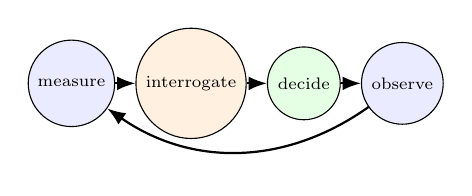
\begin{tikzpicture}[>=Latex,node distance=3mm,scale=.86,transform shape,every node/.style={font=\scriptsize,align=center}]
\node[draw,circle,fill=blue!8] (m) {measure};
\node[draw,circle,fill=orange!12,right=of m] (i) {interrogate};
\node[draw,circle,fill=green!10,right=of i] (d) {decide};
\node[draw,circle,fill=blue!8,right=of d] (o) {observe};
\draw[->,thick] (m)--(i); \draw[->,thick] (i)--(d); \draw[->,thick] (d)--(o);
\draw[->,thick,bend left=35] (o) to (m);
\end{tikzpicture}
\visualdescription{Measurement, interrogation, decision, and observation form a lifecycle.}
\slidesource{\parencite{NationalInstituteStandards2023ArtificialIntelligenceRisk}; \parencite{Phillips2026TEVVAthlon}}
\end{frame}

\section{References}
\begin{frame}[t]{References}
  \printbibliography[heading=none,category=referencesone]
\end{frame}
\begin{frame}[t]{References}
  \printbibliography[heading=none,category=referencestwo]
\end{frame}
\begin{frame}[t]{References}
  \printbibliography[heading=none,category=referencesthree]
\end{frame}
\begin{frame}[t]{References}
  \printbibliography[heading=none,category=referencesfour]
\end{frame}

\end{document}
